\documentclass{beamer}
\mode<presentation>{
  \usetheme{Boadilla}
  \usefonttheme[onlylarge]{structurebold}
  \usefonttheme[stillsansseriflarge]{serif}
  \setbeamerfont*{frametitle}{size=\normalsize,series=\bfseries}
  % \setbeamertemplate{navigation symbols}{}
  \setbeamercovered{transparent}
}
\usepackage[english]{babel}
\usepackage[latin1]{inputenc}
\usepackage{times}
\usepackage[T1]{fontenc}
\usepackage{amsmath}
\usepackage{amssymb}
\usepackage{esint}
\usepackage{hyperref}
\usepackage{tikz}
\usepackage{transparent}
\usepackage{xkeyval}
\usepackage{xargs}
\usepackage{xcolor}
\usepackage{verbatim}
\usepackage{listings}
\usepackage{multimedia}
% \usepackage{bm}
% \usepackage{siunitx}
\usepackage{ifthen}
\usepackage{enumitem}
\usepackage{stmaryrd}
\usepackage{changepage}
\setlist[itemize]{label=\textbullet}
\usetikzlibrary{
  arrows,
  calc,
  decorations.pathmorphing,
  decorations.pathreplacing,
  decorations.markings,
  fadings,
  positioning,
  shapes,
  arrows.meta
}
\usepgfmodule{oo}

\pgfdeclareradialshading{glow2}{\pgfpoint{0cm}{0cm}}{
  color(0mm)=(white);
  color(2mm)=(white);
  color(8mm)=(black);
  color(10mm)=(black)
}
\pgfdeclareradialshading{glow}{\pgfpoint{0cm}{0cm}}{
  color(0mm)=(white);
  color(5mm)=(white);
  color(9mm)=(black);
  color(10mm)=(black)
}

\begin{tikzfadingfrompicture}[name=glow fading]
  \shade [shading=glow] (0,0) circle (1);
\end{tikzfadingfrompicture}

\begin{tikzfadingfrompicture}[name=glow2 fading]
  \shade [shading=glow2] (0,0) circle (1);
\end{tikzfadingfrompicture}

\definecolor{atomorange}{rgb}{1.0,0.483,0.0}
\definecolor{pyplotc0}{rgb}{0.122,0.467,0.706}
\definecolor{pyplotc1}{rgb}{1.000,0.498,0.055}
\definecolor{pyplotc2}{rgb}{0.173,0.627,0.173}
\definecolor{pyplotc3}{rgb}{0.839,0.153,0.157}
\definecolor{pyplotc4}{rgb}{0.580,0.404,0.741}
\definecolor{pyplotc5}{rgb}{0.549,0.337,0.294}
\definecolor{pyplotc6}{rgb}{0.890,0.467,0.761}
\definecolor{pyplotc7}{rgb}{0.498,0.498,0.498}
\definecolor{pyplotc8}{rgb}{0.737,0.741,0.133}
\definecolor{pyplotc9}{rgb}{0.090,0.745,0.812}

\newcommand\drawmirror[4][line width=3]{
  % 1: draw option
  % 2: center (x, y)
  % 3: size
  % 4: angle
  \draw[#1] ($#2 + ({#3 * cos(#4)}, {#3 * sin(#4)})$) --
  ($#2 - ({#3 * cos(#4)}, {#3 * sin(#4)})$);
}

\mode<handout>{
  \usepackage{pgfpages}
  \pgfpagesuselayout{4 on 1}[a4paper,landscape,border shrink=5mm]
  \setbeamercolor{background canvas}{bg=black!10}
}

\newcommand\pgfmathsinandcos[3]{%
  \pgfmathsetmacro#1{sin(#3)}%
  \pgfmathsetmacro#2{cos(#3)}%
}
\newcommand\LongitudePlane[3][current plane]{%
  \pgfmathsinandcos\sinEl\cosEl{#2} % elevation
  \pgfmathsinandcos\sint\cost{#3} % azimuth
  \tikzset{#1/.estyle={cm={\cost,\sint*\sinEl,0,\cosEl,(0,0)}}}
}
\newcommand\LatitudePlane[3][current plane]{%
  \pgfmathsinandcos\sinEl\cosEl{#2} % elevation
  \pgfmathsinandcos\sint\cost{#3} % latitude
  \pgfmathsetmacro\yshift{\cosEl*\sint}
  \tikzset{#1/.estyle={cm={\cost,0,0,\cost*\sinEl,(0,\yshift)}}} %
}
\newcommand\DrawLongitudeCircle[2][1]{
  \LongitudePlane{\angEl}{#2}
  \tikzset{current plane/.prefix style={scale=#1}}
  % angle of "visibility"
  \pgfmathsetmacro\angVis{atan(sin(#2)*cos(\angEl)/sin(\angEl))} %
  \draw[current plane] (\angVis:1) arc (\angVis:\angVis+180:1);
  \draw[current plane,dashed] (\angVis-180:1) arc (\angVis-180:\angVis:1);
}
\newcommand\DrawLatitudeCircleArrow[2][1]{
  \LatitudePlane{\angEl}{#2}
  \tikzset{current plane/.prefix style={scale=#1}}
  \pgfmathsetmacro\sinVis{sin(#2)/cos(#2)*sin(\angEl)/cos(\angEl)}
  % angle of "visibility"
  \pgfmathsetmacro\angVis{asin(min(1,max(\sinVis,-1)))}
  \draw[current plane,decoration={markings, mark=at position 0.6 with {\arrow{<}}},postaction={decorate},line width=.6mm] (\angVis:1) arc (\angVis:-\angVis-180:1);
  \draw[current plane,dashed,line width=.6mm] (180-\angVis:1) arc (180-\angVis:\angVis:1);
}
\newcommand\DrawLatitudeCircle[2][1]{
  \LatitudePlane{\angEl}{#2}
  \tikzset{current plane/.prefix style={scale=#1}}
  \pgfmathsetmacro\sinVis{sin(#2)/cos(#2)*sin(\angEl)/cos(\angEl)}
  % angle of "visibility"
  \pgfmathsetmacro\angVis{asin(min(1,max(\sinVis,-1)))}
  \draw[current plane] (\angVis:1) arc (\angVis:-\angVis-180:1);
  \draw[current plane,dashed] (180-\angVis:1) arc (180-\angVis:\angVis:1);
}
\newcommand\coil[1]{
  {\rh * cos(\t * pi r)}, {\apart * (2 * #1 + \t) + \rv * sin(\t * pi r)}
}
\makeatletter
\define@key{DrawFromCenter}{style}[{->}]{
  \tikzset{DrawFromCenterPlane/.style={#1}}
}
\define@key{DrawFromCenter}{r}[1]{
  \def\@R{#1}
}
\define@key{DrawFromCenter}{center}[(0, 0)]{
  \def\@Center{#1}
}
\define@key{DrawFromCenter}{theta}[0]{
  \def\@Theta{#1}
}
\define@key{DrawFromCenter}{phi}[0]{
  \def\@Phi{#1}
}
\presetkeys{DrawFromCenter}{style, r, center, theta, phi}{}
\newcommand*\DrawFromCenter[1][]{
  \setkeys{DrawFromCenter}{#1}{
    \pgfmathsinandcos\sint\cost{\@Theta}
    \pgfmathsinandcos\sinp\cosp{\@Phi}
    \pgfmathsinandcos\sinA\cosA{\angEl}
    \pgfmathsetmacro\DX{\@R*\cost*\cosp}
    \pgfmathsetmacro\DY{\@R*(\cost*\sinp*\sinA+\sint*\cosA)}
    \draw[DrawFromCenterPlane] \@Center -- ++(\DX, \DY);
  }
}
\newcommand*\DrawFromCenterText[2][]{
  \setkeys{DrawFromCenter}{#1}{
    \pgfmathsinandcos\sint\cost{\@Theta}
    \pgfmathsinandcos\sinp\cosp{\@Phi}
    \pgfmathsinandcos\sinA\cosA{\angEl}
    \pgfmathsetmacro\DX{\@R*\cost*\cosp}
    \pgfmathsetmacro\DY{\@R*(\cost*\sinp*\sinA+\sint*\cosA)}
    \draw[DrawFromCenterPlane] \@Center -- ++(\DX, \DY) node {#2};
  }
}
\makeatother

% not mandatory, but I thought it was better to set it blank
\setbeamertemplate{headline}{}
\def\beamer@entrycode{\vspace{-\headheight}}

\tikzstyle{snakearrow} = [decorate, decoration={pre length=0.2cm,
  post length=0.2cm, snake, amplitude=.4mm,
  segment length=2mm},thick, ->]
\tikzstyle{fullsnakearrow} = [decorate, decoration={pre length=0cm,
  post length=0.09cm, snake, amplitude=.4mm,
  segment length=2mm},thick, ->]

%% document-wide tikz options and styles

\tikzset{%
  % >=latex, % option for nice arrows
  inner sep=0pt,%
  outer sep=2pt,%
  mark coordinate/.style={inner sep=0pt,outer sep=0pt,minimum size=3pt,
    fill=black,circle}%
}
\tikzset{
  % Define standard arrow tip
  >=stealth',
  % Define style for boxes
  punkt/.style={
    rectangle,
    rounded corners,
    draw=black, very thick,
    text width=8em,
    minimum height=2.5em,
    text centered},
}
\tikzset{
  mid arrow/.style={postaction={decorate,decoration={
        markings,
        mark=at position #1 with {\arrow[>=stealth]{>}}
      }}},
  mid arrow/.default=0.5,
  mid arrow2/.style={postaction={decorate,decoration={
        markings,
        mark=at position #1 with {\arrow[>=stealth]{><}}
      }}},
  mid arrow2/.default=0.5,
}

\tikzset{onslide/.code args={<#1>#2}{%
    \only<#1>{\pgfkeysalso{#2}}
    % \pgfkeysalso doesn't change the path
  }}
\tikzset{alt/.code args={<#1>#2#3}{%
    \alt<#1>{\pgfkeysalso{#2}}{\pgfkeysalso{#3}}
    % \pgfkeysalso doesn't change the path
  }}
\tikzset{temporal/.code args={<#1>#2#3#4}{%
    \temporal<#1>{\pgfkeysalso{#2}}{\pgfkeysalso{#3}}{\pgfkeysalso{#4}}
    % \pgfkeysalso doesn't change the path
  }}

\makeatletter
\newbox\@backgroundblock
\newenvironment{backgroundblock}[2]{%
  \global\setbox\@backgroundblock=\vbox\bgroup%
  \unvbox\@backgroundblock%
  \vbox to0pt\bgroup\vskip#2\hbox to0pt\bgroup\hskip#1\relax%
}{\egroup\egroup\egroup}
\addtobeamertemplate{background}{\box\@backgroundblock}{}
\makeatother

\ifpdf
% Ensure reproducible output
\pdfinfoomitdate=1
\pdfsuppressptexinfo=-1
\pdftrailerid{}
\hypersetup{
  pdfcreator={},
  pdfproducer={}
}
\fi

\newcommand{\todo}[1]{}

\newcommand\slideOn[1]{
  \ifthenelse{\isundefined\disableAllSlides} {
    \def\disableAllSlides{}
  }{}
  \expandafter\def\csname slide_ #1 _enable \endcsname{}
}
\newcommand\slideOff[1]{
  \expandafter\def\csname slide_ #1 _disable \endcsname{}
}
% \slideOn{}
\ifthenelse{\isundefined\disableAllSlides} {
  \newcommand\ifSlide[1]{
    \expandafter\ifcsname slide_ #1 _disable \endcsname
    \else
  }
} {
  \newcommand\ifSlide[1]{
    \expandafter\ifcsname slide_ #1 _enable \endcsname
  }
}

\title[Coherent Creation of Single Molecules]{Coherent Creation of Single Molecules from Single Atoms}
\date{}
\author{Yichao Yu}
\institute{Ni Group/Harvard}

\begin{document}

\pgfdeclarelayer{tweezer}
\pgfsetlayers{tweezer,main}
\pgfooclass{tweezer}{
  \method tweezer() {
  }
  \method drawTweezer(#1,#2,#3) {
    \begin{pgfonlayer}{tweezer}
      \shade[shading=radial,path fading=glow fading,shift={(#1,#2)},rotate=90,yscale=1,
      fill opacity=0.9,inner color=#3]
      plot[draw,samples=200,domain=-1.5:1.5] function {sqrt(0.01 + x**2 / 5)}
      -- plot[draw,samples=200,domain=1.5:-1.5] function {-sqrt(0.01 + x**2 / 5)};
    \end{pgfonlayer}
  }
  \method drawAtom(#1,#2,#3,#4) {
    \fill [#4,path fading=glow2 fading] (#1,#2) circle (#3);
  }
  \method drawNaAtom(#1,#2,#3) {
    \pgfoothis.drawAtom(#1,#2,#3,atomorange);
  }
  \method drawCsAtom(#1,#2,#3) {
    \pgfoothis.drawAtom(#1,#2,#3,blue);
  }
  \method drawNaTweezer(#1,#2) {
    \pgfoothis.drawTweezer(#1,#2,orange!35!black!30);
  }
  \method drawCsTweezer(#1,#2) {
    \pgfoothis.drawTweezer(#1,#2,blue!30!black!30);
  }
  \method up(#1,#2) {
    \pgfoothis.drawCsTweezer(#1,#2);
    \pgfoothis.drawNaAtom(#1,#2+0.06,0.12);
    \pgfoothis.drawCsAtom(#1,#2-0.06,0.16);
  }
  \method down(#1,#2) {
    \pgfoothis.drawCsTweezer(#1,#2);
    \pgfoothis.drawCsAtom(#1,#2+0.06,0.16);
    \pgfoothis.drawNaAtom(#1,#2-0.06,0.12);
  }
  \method naTrap(#1,#2) {
    \pgfoothis.drawNaTweezer(#1,#2);
    \pgfoothis.drawNaAtom(#1,#2,0.12);
  }
  \method csTrap(#1,#2) {
    \pgfoothis.drawCsTweezer(#1,#2);
    \pgfoothis.drawCsAtom(#1,#2,0.16);
  }
}
\pgfoonew \mytweezer=new tweezer()

%% Title
% Hello everyone, thanks for being here today at my thesis defense.
% I'm Yichao from the Ni lab and today I'll tell you about our experiment
% on creating single NaCs molecules in optical tweezers from atoms.
\ifSlide{title}
{
  \usebackgroundtemplate{
    \makebox[\paperwidth][c]{\centering
      \includegraphics[width=\paperwidth]{figures/title_background.png}}
  }
  \setbeamercolor{title}{fg=white}
  \setbeamercolor{author}{fg=white}
  \setbeamercolor{institute}{fg=white}
  \setbeamercolor{date}{fg=white}
  \begin{frame}{}
    \titlepage
  \end{frame}
}
\fi

%% Goal
% But before going into the details, let's first talk about why we want to do this. __(>>2>>)__
% __(1/00:20)__

% One of the most popular paradigms in AMO,
% that is atomic, molecular and optical physics,
% is to take very simple and well understood systems,
% apply really high degree of control based on our understanding of it
% in order to realize and study very complex dynamics
% or other interesting processes that emerges from them. __(>>)__
% As probably the most well known examples in this field,
% using the simplest atoms in the world other than Hydrogen, namely Alkali atoms,
% by precisely controlling these simple atoms,
% people were able to realize whole new quantum phases of matter,
% so-called Bose-Einstein condensate,
% and even putting them in a lattice structure
% to simulate solid state systems and
% to further our understanding on some of the mysteries
% such as magnetism or high temperature superconductors.
% __(2/01:20)__

% But of course we aren't satisfied with only the simplest system
% and there're good reasons for that. __(>>)__
% The neutral atomic systems are, well, too simple.
% And more precisely what I meant is that they have relatively simple internal structures
% and they really don't want to interact with other atoms.
% As you might imagine by making an analogy with social interactions,
% it's hard to convince these atoms to behave collectively
% and have interesting dynamics within the group.
% Certainly possible as I previously shown, just difficult,
% and the achievement done with atoms really make one wonder what would be possible
% if we could have a system that is simple enough to control
% but also complex enough to make it easier to do interesting stuff.
% So, with that in mind, let's make a simple checklist for an ideal system shall we? __(>>)__
% __(3/02:25)__

% * First, as I said, it must have strong interaction and preferably a long range one. __(>>)__
% * Related to that, it should have a long coherence time,
% % at least compared to the speed of the interaction,
% % so that we can do useful things with it before it dies. __(>>)__
% * Next, also mentioned before, we would like a rich internal structure.
% % These give us more flexibility, allow more interesting dynamics to occure
% % and will also be our knobs to tune the systems. __<span style="color:red">(>>)</span>__
% * And finally, we don't want to give up on our control.
% % If we couldn't prepare the system and ask it to do exactly what we want,
% % it's easy to see why this would makes it kinda hard to use the system to do anything useful.
% __(4/03:10)__

% I have to say that of course we didn't come up with this list
% and we are not the only one that explore new options.
% In fact neutral atom isn't even the first system people used. __(>>)__
% There are many other choices for example like ions and Rydberg atoms.
% Nevertheless, I believe it is still worth investigating in new systems like what we do,
% because first, all of the existing systems still have their limitations
% and although I'll not claim that we fixed all those issues
% and have the best system in the world, at least not yet, __(>>)__
% we do have our unique properties and different trade offs
% which I'll breifly talk about later.
% In the mean time, we are also bringing in new solutions and tools to the field
% and in fact some of the new techniques I'll mention today,
% should be applicable and are being applied to many other systems.
% __(5/04:15)__
\ifSlide{intro_motivation}
\begin{frame}{}
  \begin{center}
    \begin{tikzpicture}
      \begin{scope}[shift={(-1.5, 2)}]
        \node at (0, 0) {Simple System};
        \mytweezer.drawCsAtom(-0.7, -0.8, 0.15)
        \mytweezer.drawCsAtom(0.6, -0.9, 0.15)
        \mytweezer.drawNaAtom(-0.1, -0.7, 0.21)
      \end{scope}

      \begin{scope}[shift={(1.4, 2)}]
        \node at (0, 0) {Full Control};
        \mytweezer.drawCsAtom(-0.4, -1, 0.15)
        \draw[fullsnakearrow,>=stealth,red]
        (-0.4 - 0.9, -1 + 0.6) -- (-0.4 - 0.09, -1 + 0.06);
        \mytweezer.drawNaAtom(0.5, -0.8, 0.21)
        \draw[->,>=latex,green!70!black,thick] (-0.1, -0.35) -- ++(1.3, 0);
        \draw[->,>=latex,green!70!black,thick] (-0.1, -0.65) -- ++(1.3, 0);
        \draw[->,>=latex,green!70!black,thick] (-0.1, -0.95) -- ++(1.3, 0);
        \draw[->,>=latex,green!70!black,thick] (-0.1, -1.25) -- ++(1.3, 0);
      \end{scope}
      \draw[decoration={brace,mirror,raise=3pt, amplitude=10pt},decorate,line width=2]
      (-2.5, 0.6) -- node[below=0.5] {Complex Dynamic} (2.5, 0.6);
      \visible<2->{
        \node[below,align=center] at (-1.4, -0.5) {
          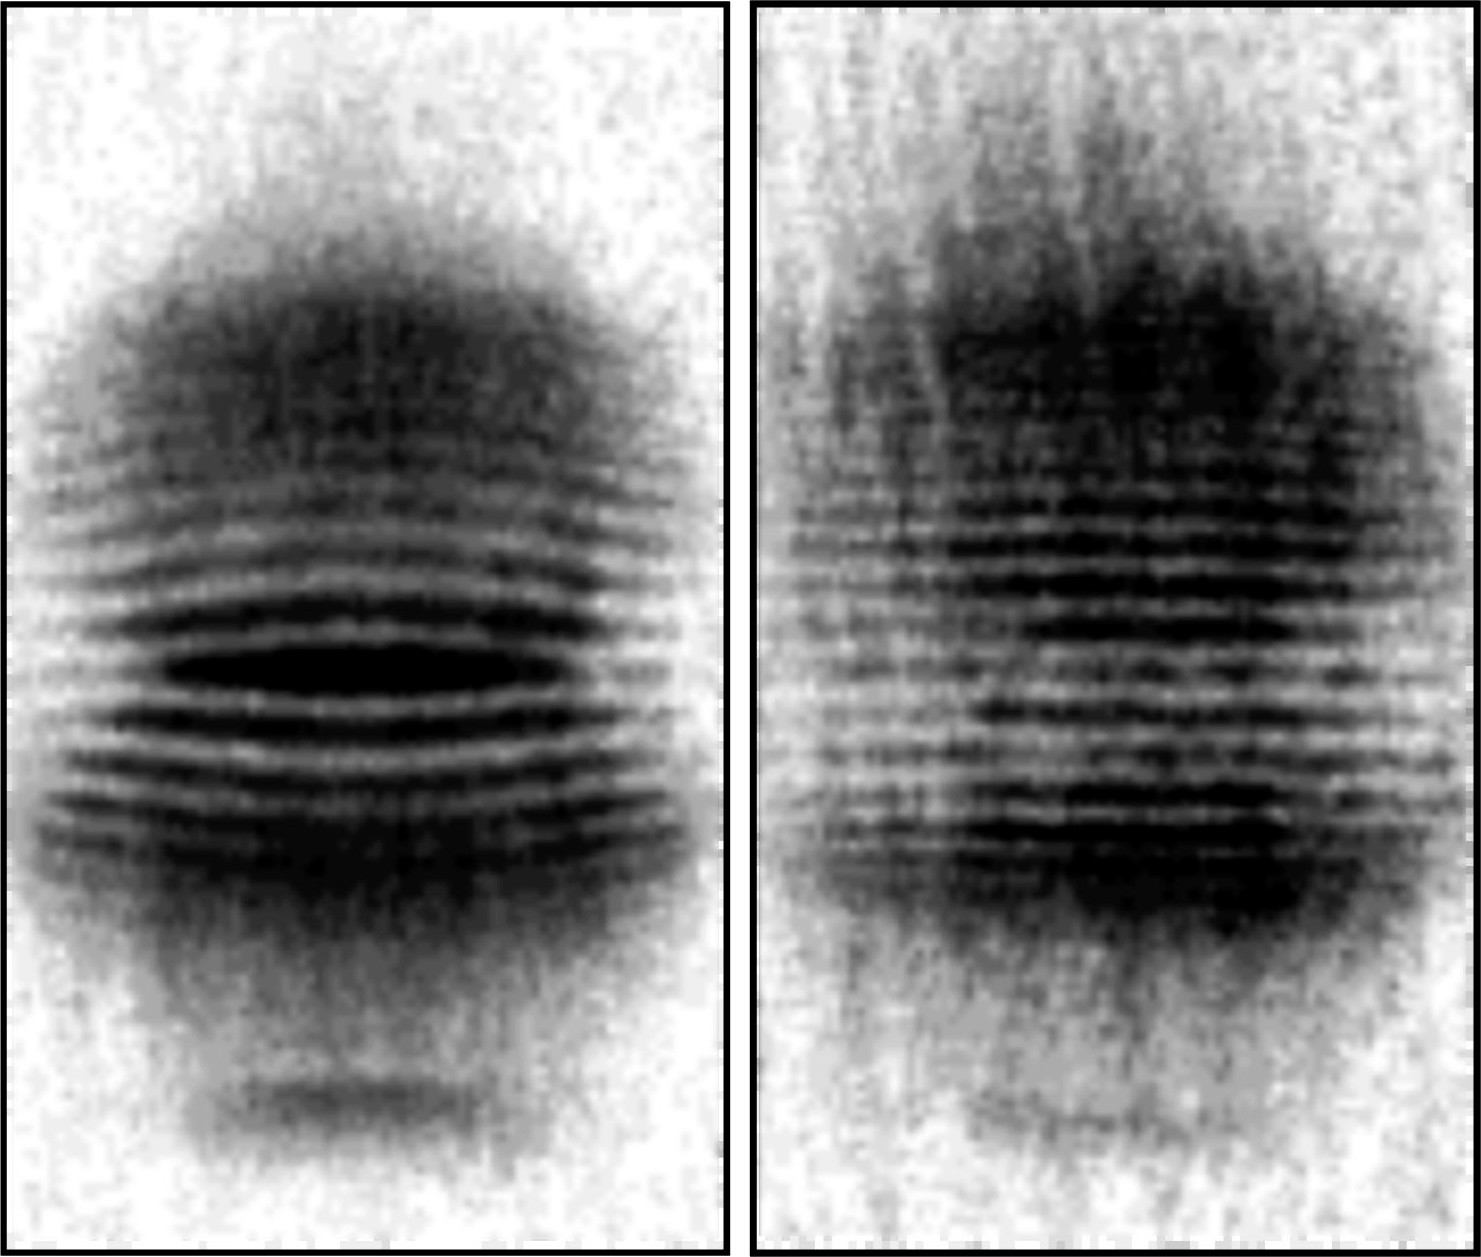
\includegraphics[width=2.7cm]{figures/introduction_atom_bec_interference.png}\\
          {\tiny Science  275, 637 (1997)}};
        \node[below,align=center] at (1.4, -0.5) {
          \includegraphics[width=2.7cm]{figures/introduction_lithium_microscope.png}\\
          {\tiny Nature 545, 462-466 (2017)}};
      }
      \visible<3->{
        \node[below,align=center,text width=5cm] at (0, -4) {
          \begin{itemize}[label={\textcolor{red}{$\times$}}]
          \item Simple internal structure
          \item Weak interaction
          \end{itemize}
        };
      }
      \visible<4->{
        \node[below,align=center,text width=5cm] at (6, 2.8) {
          \begin{itemize}[label=$\boxempty$]
          \item Strong interaction
          \item<5-> Long coherence time
          \item<6-> Rich internal structure
          \item<7-> Fully controllable
          \end{itemize}
        };
      }
      \visible<8->{
        \node[below,align=center] at (6.2, -0.5) {
          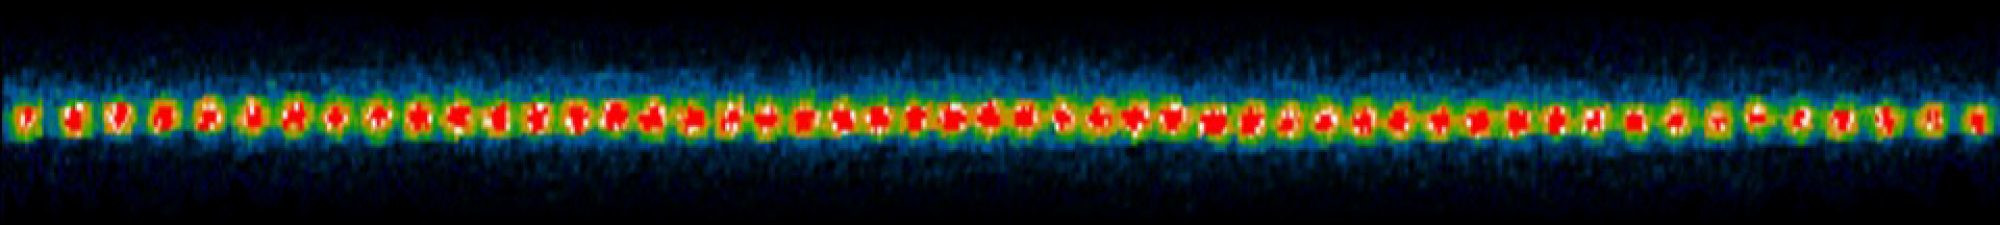
\includegraphics[width=5cm]{figures/introduction_ion_chain.jpg}\\
          Ions {\tiny (Photo credit: Monroe group)}};
        \node[below,align=center] at (6.2, -1.9) {
          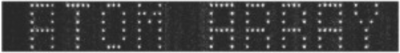
\includegraphics[width=5cm]{figures/introduction_atom_array.png}\\
          Rydberg Atoms {\tiny (Photo credit: Lukin group)}};
      }
      \visible<8>{
        \node[below,align=center] at (6.2, -3.6)
        {\usebeamercolor[fg]{frametitle}{\bf \phantom{?}New System?}};
      }
      \visible<9->{
        \node[below,align=center] at (6.2, -3.6)
        {\usebeamercolor[fg]{frametitle}{\bf \phantom{!}New System!}};
        \node[below,align=center,text width=5cm] at (6.2, -3.9)
        {
          \begin{itemize}
          \item Different properties
          \item New tools and techniques
          \end{itemize}
        };
      }
    \end{tikzpicture}
  \end{center}
\end{frame}
\fi

%% System
% So now let's look at our system selection. __(>>3>>)__

% I've shown this checklist with a few requirements
% and let's start with the strong interaction. __(>>)__
% Well, this requirement is the main reason we chose dipole molecules
% as you've seen from the title.
% Compared to neutral atoms, they have much stronger and longer range interactions,
% roughly `kHz` about a micron apart allowing faster entanglement or gate operations.
% Additionally, the interacting molecules are long lived
% and the interaction between them are easily tunable.
% These somewhat unique combination of properties are very useful
% for reducing the coupling with the enviroment and achieving long coherence time,
% so that's another check. __(>>)__
% As a bonus, molecules also have rich internal states,
% which is actually the main reason for the tunability of interaction, __(>>)__
% and it give us the flexibility I mentioned earlier,
% for example in the selection of qubit states for quantum information applications.
% __(6/05:30)__

% The one item left now is full quantum control,
% and for that our main tool is the optical tweezer. __(>>)__
% This is created by focusing a light beam to a really small spot
% such that the intensity of the light is strong enough to trap a single particle,
% similar to, well, a tweezer. __(>>)__
% Since it is form by focusing light onto a small spot,
% the optics to do so very naturally gives us the resolution to see that spot
% and to detect and manipulate the single molecule trapped there,
% hense giving us the full control we need.
% This technique has been developed in many other groups for atoms
% including Lukin group here at Harvard. __(>>)__
% People have demostrated sideband cooling, near deterministic loading
% and even flexible rearrangment of the tweezers.
% In our experiment, we would like to extend these capabilities from atoms to molecules
% and you'll see later in my talk how we use this
% to achieve quantum control on the molcules we create.
% __(7/06:45)__
\ifSlide{intro_system}
\begin{frame}{}
  \begin{center}
    \begin{tikzpicture}
      \node[below,align=center,text width=5.5cm] at (-3, 2.2) {
        \begin{itemize}[label=$\boxempty$]
        \item[\alt<2->{\textcolor{green!70!black}{\checkmark}}{$\boxempty$}]
          Strong interaction \textcolor{red}{\visible<2->{(kHz)}}
        \item[\alt<3->{\textcolor{green!70!black}{\checkmark}}{$\boxempty$}]
          Long coherence time
        \item[\alt<4->{\textcolor{green!70!black}{\checkmark}}{$\boxempty$}]
          Rich internal structure
        \item[\alt<5->{\textcolor{green!70!black}{\checkmark}}{$\boxempty$}]
          Fully controllable
        \end{itemize}
      };
      \visible<-6>{
        \node[below,align=center] at (-3, -0.7) {
          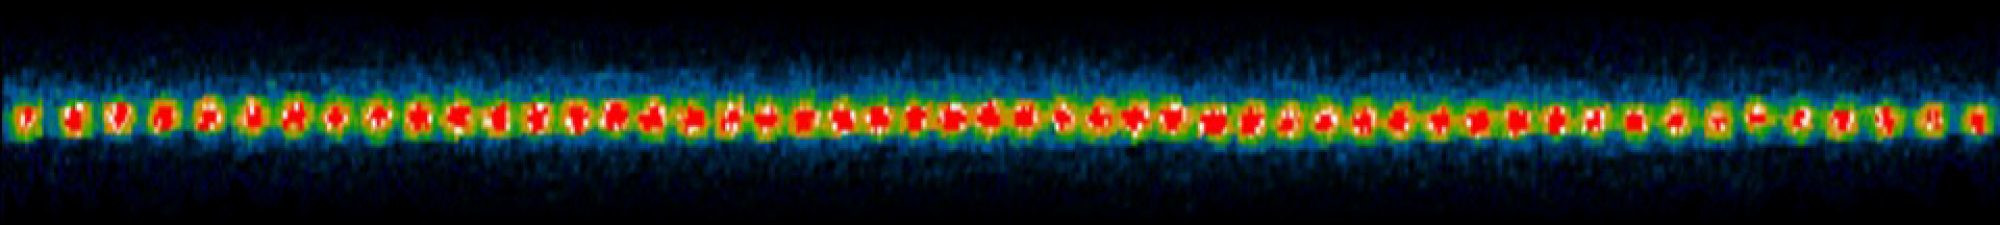
\includegraphics[width=5cm]{figures/introduction_ion_chain.jpg}\\
          Ions {\tiny (Photo credit: Monroe group)}};
        \node[below,align=center] at (-3, -2.1) {
          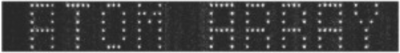
\includegraphics[width=5cm]{figures/introduction_atom_array.png}\\
          Rydberg Atoms {\tiny (Photo credit: Lukin group)}};
        \visible<2->{
          \node[below,align=center] at (-3, -3.6) {
            \includegraphics[width=5.2cm]{figures/introduction_molecule_quantum_computing.pdf}\\
            {\usebeamercolor[fg]{frametitle}{Dipolar Molecule}}
            {\tiny (Chemical Science 9, 6830 - 6838 (2018))}};
        }
      }
      \visible<5->{
        \node[below,align=center,text width=5.8cm] at (3, 1.8) {{
            {\usebeamercolor[fg]{frametitle}{\textbf{Optical tweezers}}}
            \begin{itemize}
            \item<6-> Single site resolution
            \item<7-> $\cdots$
            \end{itemize}
          }};
      }
      \visible<7->{
        \node[align=center] at (-3.3, -3) {
          \usebeamercolor[fg]{frametitle}{\footnotesize Loading}\\
          \includegraphics[width=3.8cm]{figures/introduction_tweezer_loading.pdf}\\
          {\tiny Nat. Phys. 6, 951 (2010)}
        };
        \node[align=center] at (2.7, -1.2) {
          \usebeamercolor[fg]{frametitle}{\footnotesize Cooling}\\
          \includegraphics[width=3.5cm]{figures/introduction_tweezer_rsc.pdf}\\
          {\tiny PRX. 2, 041014 (2012)}
        };
        \node[align=center] at (2.4, -4.5) {
          \usebeamercolor[fg]{frametitle}{\footnotesize Rearranging}\\
          \includegraphics[width=5.7cm]{figures/introduction_tweezer_rearrange.png}\\
          {\tiny Science 354, 1024 (2016)}
        };
      }
    \end{tikzpicture}
  \end{center}
\end{frame}
\fi

%% Molecules in tweezers
% So since our goal is to create ultracold molecules,
% there are basically two ways to do this. __(>>4>>)__
% One approach is to first get molecule and then get ultracold,
% in another word, direct cooling of hot molecules to ultracold temperature
% without destroying or otherwise loosing the molecule in that process.
% This is a very hard problem even without loading into optical tweezer
% because of the difficulties in laser cooling,
% but there has been a lot of progress in this area.
% In fact, the Doyle group at Harvard have demostrated almost two years ago
% trapping ultracold CaF molecules in an array of optical tweezers,
% as you can see in this picture.
% __(8/07:35)__

% The other approach, which is what we use, __(>>)__
% is to get ultracold, and then get molecule.
% In another word, we would cool and fully control the atoms,
% before turning them into molecules coherently,
% without heating them, and in general maintaining the control we had
% on the atoms in this process.
% __(9/08:00)__

% Comparing the two approaches, __(>>)__
% the main challenge currently for the direct cooling approach
% is to cool and in general controlling the molecules in the tweezer.
% Whereas for us, __(>>)__ what we have to do is to first establish the control on the atoms
% and then create our molecules from the atoms coherently.
% These two points will be what I'm going to focus on for the remainder of my talk
% __(10/08:30)__
\ifSlide{intro_molecule_tweezer}
\begin{frame}{Ultracold molecules in tweezers}
  \begin{center}
    \begin{tikzpicture}
      \uncover<-3>{
        \node at (-3, 4) {\usebeamercolor[fg]{frametitle}{\textbf{Direct cooling}}};
      }
      \node[below, align=center] (CaFnode) at (-3, 3.5) {
        \includegraphics[width=6cm]{figures/introduction_caf_tweezer.png}\\
        \vspace{0.5cm}
        {\tiny Science 365, 1156 (2019)}
      };
      \visible<4->{
        \fill[white,opacity=0.9] (CaFnode.north west) rectangle (CaFnode.south east);
      }

      \visible<2->{
        \uncover<2,4->{
          \node at (3, 4) {\usebeamercolor[fg]{frametitle}{\textbf{Assembly}}};
          \begin{scope}[shift={(1.6, 3.2)}, scale=0.5]
            \shade[ball color=blue!90] (-0.8, 0.2) circle (0.45);
            \shade[ball color=orange!90] (0.3, -0.2) circle (0.3);
          \end{scope}
          \node[align=center] (atom) at (3, 3.2) {\hspace{1cm}\textbf{Ultracold atoms}};
          \begin{scope}[shift={(1.35, 1.5)}, scale=0.5]
            \shade[ball color=blue!90] (-0.2, -0.1) circle (0.45);
            \shade[ball color=orange!90] (0.2, 0.1) circle (0.3);
          \end{scope}
          \node[align=center] (molecule) at (3, 1.5) {\hspace{1cm}\textbf{Ultracold molecule}};
          \draw[blue,->,line width=2,>=stealth] (atom) --
          node[right] {\small \textbf{Coherent transfer}} (molecule);
        }
      }

      \visible<3->{
        \node at (0, 0) {\usebeamercolor[fg]{frametitle}{\underline{\textbf{Challenges}}}};
      }

      \visible<3->{
        \uncover<3>{
          \node[below, text width=5.5cm, align=left] at (-3, -0.8) {\begin{itemize}
            \item Temperature in tweezer
            \item Quantum control
            \end{itemize}};
        }
      }

      \visible<4->{
        \node[below, text width=4cm, align=left] at (3, -0.7) {\begin{itemize}
          \item Control of atoms
          \item Coherent creation of molecules
          \end{itemize}};
      }
    \end{tikzpicture}
  \end{center}
\end{frame}
\fi

%% Outline
% __(>>5>>)__ So here's an outline for the rest of my talk.
% I'll first give an overview of our experiment, both the procedure and the apparatus.
% Then as one example of achieving full control on our atoms,
% I'll discuss the cooling of Na atom in the tweezer.
% After that I'll describe our measurement of the interaction between atoms
% both to demostrate what control we have
% and as a preparation for our molecule formation.
% And finally I'll talk about how we create the molecules coherently,
% before giving my conclusion.
% __(11/09:15)__
\ifSlide{outline}
\begin{frame}{Outline}
  \tableofcontents
\end{frame}
\fi

\section{Experiment overview}
%% Experiment overview
% So first the experiment. __(>>6>>)__ The molecules we make is NaCs, chosen because
% a) it is fromed by two alkali atoms which are relatively easy to cool and control,
% and b) this molecule has a fairly strong dipole moment of 4.6 debye
% among the bi-alkalis and even many other diatomic molecules,
% which give rise to the strong interaction we need.
% __(12/09:45)__
\ifSlide{overview_molecule}
\begin{frame}[t]{Experiment overview}
  \begin{columns}
    \column{5.8cm}
    \column{5.8cm}
    \begin{center}
      {\usebeamerfont{frametitle}\usebeamercolor[fg]{frametitle}{\Large NaCs molecule}}\\
      \begin{itemize}
      \item Bi-alkali (easy to control)
      \item Large dipole moment: $4.6~\mathrm{D}$
      \end{itemize}
    \end{center}
  \end{columns}
\end{frame}
\fi

% Since we are making molecules from atoms inside the optical tweezer,
% the obvious first step is to get the atoms in there. __(>>7>>)__
% This has been done previously for Rb in other group.
% And while doing this for Cs was relatively straightforward,
% getting this working for Na had some difficulties related to the light shift from the tweezer
% that we have to overcome by switching the tweezer on and off.
% After figuring that out, we can now trap the atoms
% in their respective tweezers directly from the MOT
% as you can see in this picture, with about 60% loading probability.
% __(13/10:30)__

% __(>>)__ We then prepare the initial state for the atoms, both internal and motional,
% using optical pumping and Raman sideband cooling to a single quantum state
% with a fairly high fidelity.
% And I'll talk about how we do this for Na in more detail later.
% __(14/10:50)__

% At this point the atoms are still in their own tweezers,
% which isn't very helpful for making a single molecule,
% since they are so far apart and can't see or feel each other. __(>>)__
% So the natural next step is to move one of the tweezers
% and merge the two atoms into the same one.
% We do this in a way that minimize the heating to the two atoms
% so they remain in their motional ground states that we cooled them into.
% __(15/11:25)__

% __(>>)__ After the merge, the two atoms are now in the same trap
% and we proceed to measure their interaction and form the molecule from this state.
% Here are some of the results that I'll discuss in detail in the second half of my talk
% and you can also see the cover for one of our first results on making molecules.
% It shows our vacuum chamber within which all of these processes take place.
% __(16/11:55)__
\ifSlide{overview_procedure}
\begin{frame}[t]{Experiment overview}
  \vspace{-0.9cm}
  \begin{center}
    \begin{tikzpicture}[scale=0.7]
      \draw[white] (0, 0) -- (-3, 0);
      \mytweezer.drawCsTweezer(0, 0)
      \mytweezer.drawNaTweezer(-1, 0)
      \mytweezer.drawCsAtom(-0.07, 0.08, 0.22)
      \mytweezer.drawNaAtom(-1.06, -0.09, 0.27)

      \mytweezer.drawCsTweezer(0, -3.1)
      \mytweezer.drawNaTweezer(-1, -3.1)
      \mytweezer.drawCsAtom(0.0, -3.1, 0.12)
      \mytweezer.drawNaAtom(-1.0, -3.1, 0.16)

      \mytweezer.drawCsTweezer(-1, -7.0)
      \mytweezer.drawNaAtom(-1.05, -6.87, 0.16)
      \mytweezer.drawCsAtom(-0.95, -7.13, 0.12)

      \fill[white,temporal=<1>{opacity=0.82}{opacity=0}{opacity=0.5}]
      (-1.5, 1.5) rectangle (0.5, -1.5);
      \fill[white,temporal=<2>{opacity=0.82}{opacity=0}{opacity=0.5}]
      (-1.5, 1.5 - 3.1) rectangle (0.5, -1.5 - 3.1);
      \fill[white,temporal=<3-4>{opacity=0.82}{opacity=0}{opacity=0.5}]
      (-1.5, 1.5 - 7.0) rectangle (-0.5, -1.5 - 7.0);

      \visible<2->{
        \begin{scope}[alt=<2>{opacity=0.7}{opacity=0.35}]
          \draw[atomorange,dotted,line width=1.2] (-1, -0.4) -- (-1, -2.9);
          \draw[blue,dotted,line width=1.2] (0, -0.15) -- (0, -2.9);
        \end{scope}
      }

      \visible<3->{
        \begin{scope}[alt=<3>{opacity=0.7}{opacity=0.35}]
          \draw[->,>=stealth,atomorange,line width=1.2] (-1, -3.3) -- (-1, -6.7);
          \draw[->,>=stealth,blue,domain=-3.3:-6.7,smooth,variable=\y,line width=1.2]
          plot ({atan((\y+4.7) * 5) / 170 - 0.5},{\y});
        \end{scope}
      }

      \visible<1>{
        \draw[red,dashed,line width=0.5] (-1.5, -1.3) rectangle (0.5, 1.3);
        \begin{scope}[shift={(1, 1)}]
          \node[above,align=center] at (7, 0)
          {\usebeamerfont{frametitle}\usebeamercolor[fg]{frametitle}{\Large Loading}};
          \node[below,align=center] at (6.5, -0.5)
          {\includegraphics[width=5cm]{figures/overview_single_atom.png}};
          \node[below,align=center] at (7, -7.5)
          {Loading probability per site: 60\%\\
            Post select on initial and final state.};
        \end{scope}
      }
      \visible<2>{
        \draw[red,dashed,line width=0.5] (-1.5, -3.4) rectangle (0.5, 0.3);
        \begin{scope}[shift={(1, 1)}]
          \node[above,align=center] at (7, 0)
          {\usebeamerfont{frametitle}\usebeamercolor[fg]{frametitle}{\Large Cooling}};
          \node[below] at (6.5, -1)
          {\includegraphics[width=6cm]{figures/rsc_spectrum_az.pdf}};
          \only<2>{
            \node[below,align=center] at (7, -7)
            {Cs: 96\% ground state\footnote{\textbf{Y. Yu} et al. PRX 9, 021039 (2019)}\\
              Na: 94\% ground state\footnote{\textbf{Y. Yu} et al. PRA 97, 063423 (2018)}};
          }
        \end{scope}
      }
      \visible<3>{
        \draw[red,dashed,line width=0.5] (-1.5, -7.35) rectangle (0.5, -2.9);
        \begin{scope}[shift={(1, 1)}]
          \node[above,align=center] at (7, 0)
          {\usebeamerfont{frametitle}\usebeamercolor[fg]{frametitle}{\Large Merging}};
          \draw[atomorange,line width=1.5] plot[draw,samples=200,domain=4.5:10.5]
          function {-0.22 * exp(-(x - 9)**2 / 0.75**2) + -0.4 * exp(-(x - 6)**2 / 0.75**2) - 1};
          \draw[blue,line width=1.5] plot[draw,samples=200,domain=4.5:10.5]
          function {-1.2 * exp(-(x - 9)**2 / 0.75**2) + 0.45 * exp(-(x - 6)**2 / 0.75**2) - 1};
          \mytweezer.drawNaAtom(6, -1.22, 0.15)
          \mytweezer.drawCsAtom(9, -2.06, 0.11)

          \draw[atomorange,line width=1.5] plot[draw,samples=200,domain=4.5:10]
          function {-0.22 * exp(-(x - 7.5)**2 / 0.75**2)
            + -0.4 * exp(-(x - 6)**2 / 0.75**2) - 3.5};
          \draw[blue,line width=1.5] plot[draw,samples=200,domain=4.5:10]
          function {-1.2 * exp(-(x - 7.5)**2 / 0.75**2)
            + 0.45 * exp(-(x - 6)**2 / 0.75**2) - 3.5};
          \mytweezer.drawNaAtom(6, -3.72, 0.15)
          \mytweezer.drawCsAtom(7.5, -4.56, 0.11)

          \draw[atomorange,line width=1.5] plot[draw,samples=200,domain=4.5:8.5]
          function {-0.22 * exp(-(x - 6)**2 / 0.75**2) + -0.4 * exp(-(x - 6)**2 / 0.75**2) - 6};
          \draw[blue,line width=1.5] plot[draw,samples=200,domain=4.5:8.5]
          function {-1.2 * exp(-(x - 6)**2 / 0.75**2) + 0.45 * exp(-(x - 6)**2 / 0.75**2) - 6};
          \mytweezer.drawNaAtom(5.9, -6.42, 0.12)
          \mytweezer.drawCsAtom(6.05, -6.6, 0.13)

          \draw[atomorange,line width=1.5] plot[draw,samples=200,domain=4.5:8.5]
          function {-0.22 * exp(-(x - 6)**2 / 0.75**2) - 8.5};
          \draw[blue,line width=1.5] plot[draw,samples=200,domain=4.5:8.5]
          function {-1.2 * exp(-(x - 6)**2 / 0.75**2) - 8.5};
          \mytweezer.drawNaAtom(6, -8.55, 0.14)
          \mytweezer.drawCsAtom(6, -9.56, 0.11)
        \end{scope}

        \draw[dotted,line width=2,black!30,opacity=10] (0.5, -2.9) -- (4.5 + 1, -0.5 + 1);
        \draw[dotted,line width=2,black!30,opacity=10] (0.5, -7.35) -- (4.5 + 1, -9.3 + 1);
      }
      \visible<4>{
        \draw[red,dashed,line width=0.5] (-1.5, -8.3) rectangle (-0.5, -5.7);
        \node (Interaction) at (4, 0)
        {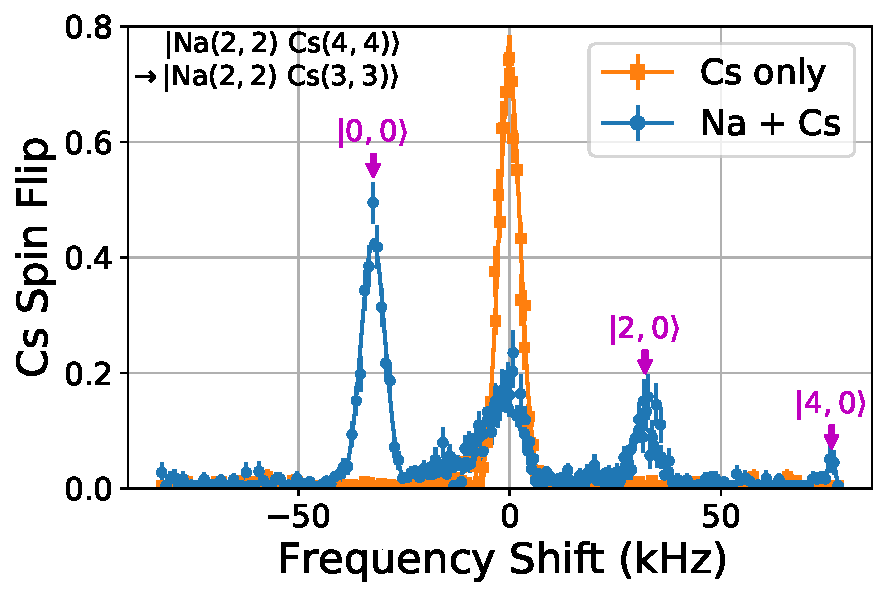
\includegraphics[width=4cm]{figures/interaction_shift_spectrum_42_32.pdf}};
        \node[above=-0.1] at ($(Interaction.north) + (0.4, 0)$)
        {\usebeamercolor[fg]{frametitle}{Interaction}};
        \node[below=-0.1] at ($(Interaction.south) + (0.4, 0)$)
        {\tiny Phys. Rev. Research 2, 023108 (2020)};
        \node (Molecule) at (10, 0.2)
        {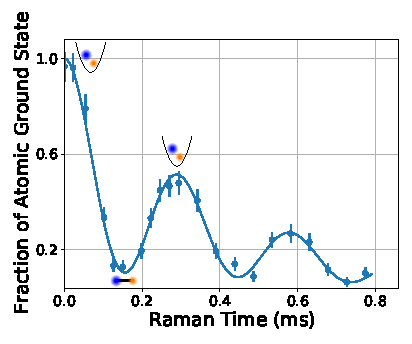
\includegraphics[width=4cm]{figures/raman_transfer_rabi_annotate.pdf}};
        \node[above=-0.35] at ($(Molecule.north) + (0.3, 0)$)
        {\usebeamercolor[fg]{frametitle}{Molecule Creation}};
        \node[align=center,
        execute at begin node=\setlength{\baselineskip}{7pt}] at (8, -6)
        {\includegraphics[width=3cm]{figures/overview_science_cover.png}\\
          \tiny L. R. Liu, J. D. Hood, \textbf{Y. Yu} et al.,\\
          \tiny Science 360, 6391 (2018)};
      }
    \end{tikzpicture}
    \vspace{-2cm}
  \end{center}
\end{frame}
\fi

%% Lab pictures
% ... which is a nice segway to talk about our apparatus
% especially since in real world, with things around the chamber, __(>>8>>)__
% this is what the experiment looks like and you can't easily see the glass cell anymore.
% Since we don't need to trap a lot of atoms and we also don't use any strong field,
% our experiment is relatively small and compact,
% at least compared to traditional bulk gas experiments. __(>>)__
% Our whole vacuum chamber is in this region surrounded by the magnetic field coil.
% It's hard to see in this picture, __(>>)__
% but from a different angle it's actually still possible to see our Na MOT
% glowing yellow in it like this which is quite amazing. __(>>)__
% Surrounding the camber we have our beam path for free space cooling, shown here, __(>>)__
% and our tweezer and imaging beam paths, here,
% as well as many others around that I won't point out one by one.
% __(17/13:00)__
\ifSlide{overview_apparatus}
\begin{frame}{}
  \begin{center}
    \begin{tikzpicture}
      \visible<1>{
        \node at (-3, 0) {\includegraphics[width=9cm]{figures/overview_chamber.png}};
      }
      \visible<2-3>{
        \node at (-3, 0) {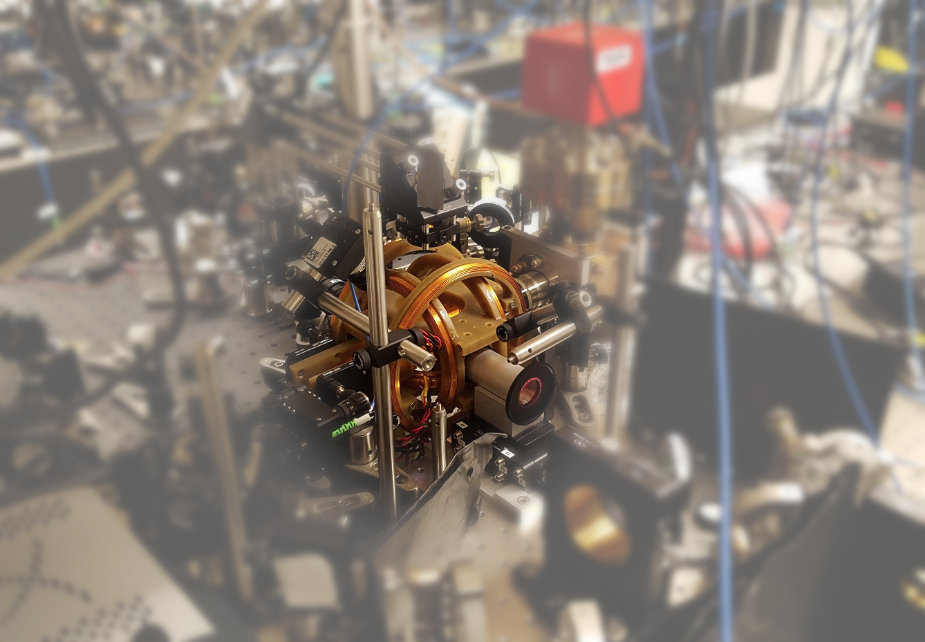
\includegraphics[width=9cm]{figures/overview_chamber_center.png}};
      }
      \visible<4>{
        \node at (-3, 3.5) {\usebeamercolor[fg]{frametitle}{\textbf{MOT beam path}}};
        \node at (-3, 0) {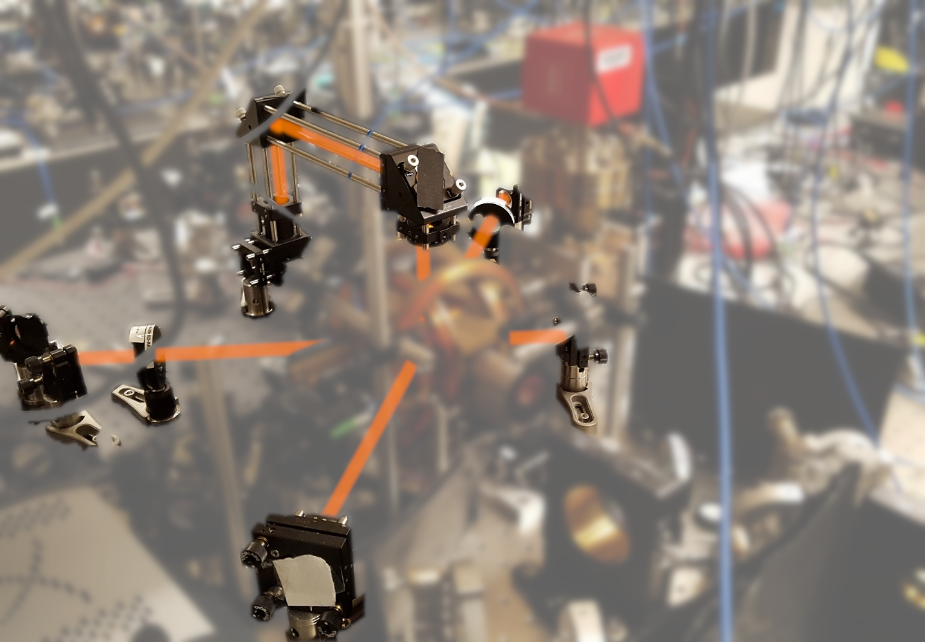
\includegraphics[width=9cm]{figures/overview_chamber_mot.png}};
      }
      \visible<5>{
        \node at (-3, 3.5)
        {\usebeamercolor[fg]{frametitle}{\textbf{Tweezer and imaging beam path}}};
        \node at (-3, 0) {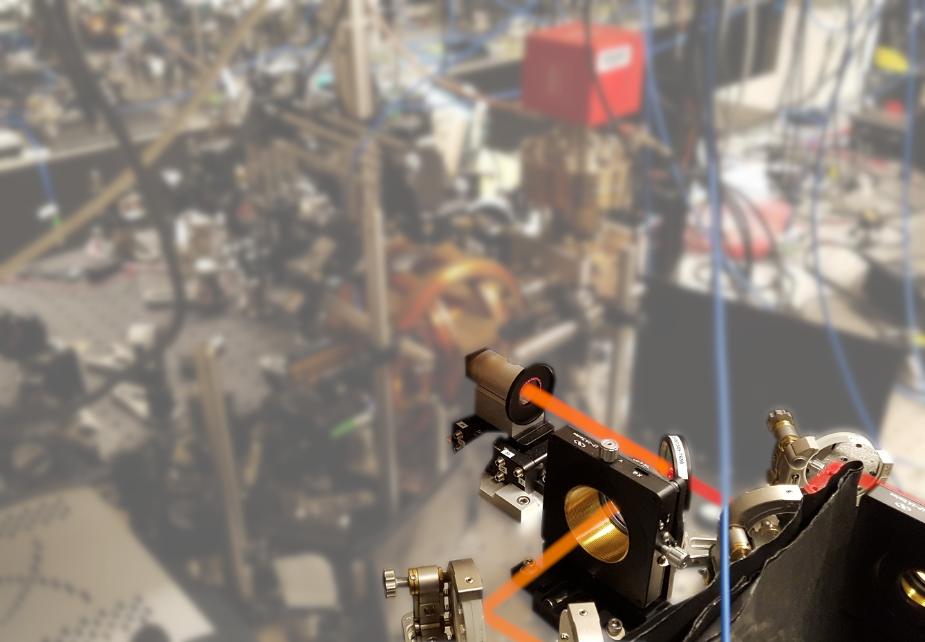
\includegraphics[width=9cm]{figures/overview_chamber_tweezer.png}};
      }
      \visible<3> {
        \draw[white, line width=2] (-3.1, -0.2) ellipse (0.25 and 0.4);
        \draw[white, line width=1.5] (-3.15, 0.2) -- (-0.5, 1.65);
        \draw[white, line width=1.5] (-3.15, -0.6) -- (-0.5, -1.65);
        \draw[white, line width=3] (-0.5, 1.65) rectangle (4.5, -1.65);
        \node at (2, 0) {\includegraphics[width=5cm]{figures/overview_na_mot.png}};
        \fill[black, opacity = 0.3, even odd rule]
        (-0.5, 1.65) rectangle (4.5, -1.65) (1.9, 0.35) circle (0.3);
        \node[below, white] at (1.9, -0.1) {\textbf{\small Na MOT}};
      }
    \end{tikzpicture}
  \end{center}
\end{frame}
\fi

\section{Atom state control}
\subsection{Raman sideband cooling of Na atoms}
%% Atom control
% So that's a rough overview of our experiment. __(>>9>>)__
% And next I'll talk about how we achieve full quantum control of our atoms,
% which, if you recall, is necessary before we can do anything coherent about molecules.
% Of course, even for atoms, there are quite a few degrees of freedoms to control
% and I don't have time to talk about every single one of them.
% So instead, I'm just going to focus on how we use Raman sideband cooling to cool Na atoms.
% __(18/13:35)__
\ifSlide{rsc_outline}
\begin{frame}{Outline}
  \tableofcontents[currentsection,currentsubsection]
\end{frame}
\fi

%% Raman sideband cooling
% __(>>10>>)__ So Raman sideband cooling is a technique for cooling particles,
% for example ion/atom/molecules etc., that is trapped in some potential.
% I imagine a lot of people here know something about it
% since it's used or is considered to be used in quite a few experiments in CUA.
% So I'm going to focus more on the differences
% and unique challenges we faced in our experiment.
% I'll talk about how we overcome these challenges
% and open up this tool to ours and other systems
% and it will hopefully be interesting for people
% who already know about Raman sideband cooling. __(>>)__
% Nevertheless, let me give a short description of how it works
% so that we can be on the same page when I talk about the difficulties we faced.
% __(19/14:25)__

% So to start here is the motional levels of an atom in a harmonic potential,
% which approximate our optical tweezer. __(>>)__
% These also exist for other spin states which we can drive to,
% say, with a Raman transitions.
% Now, due to the discrete motional levels,
% in additional to driving a "carrier" Raman transition
% at the normal resonance frequency __(>>)__ in the middle,
% with enough resolution, we can detune from it to drive "sideband" transitions
% that changes the motional state in additional to the spin states.
% When we drive the transition on the sideband,
% we can now either add, or remove motional energy from the atoms
% using the heating or cooling sidebands,
% and it is easy to see how this capability can be useful for cooling.
% __(20/)__

% Moreover, this is actually also a tool to measure the temperature of the atoms. __(>>)__
% As you can see here, the cooling sideband does not exist for all the levels,
% in particular not the ground level
% causing a reduction in its height compared to the heating sideband.
% As the temperature of the atoms get lower and lower
% and more atoms accumulate in the ground level, __(>>)__
% the cooling sideband will be more and more surpressed
% and this change in the assymetry between the two sidebands can be used
% to infer the temperature of the atom, so-called, sideband thermometry.
% __(21/)__

% Of course, this sideband transition only remove a very limited amount of energy from the atoms
% and we have to go back to the original spin state to restart the process.
% This is done using an optical pumping step __(>>)__
% which is also the step that removes the entropy, if that's your preferred picture.
% A simplified schematics of the whole cooling process is shown here
% which allows cooling the atom from arbitrary initial motional state
% all the way to the ground state following this ladder of transitions.
% __(22/16:45)__
\ifSlide{rsc_theory}
\begin{frame}{Raman sideband cooling}
  \vspace{-0.3cm}
  \begin{center}
    \begin{tikzpicture}
      \node[below,align=center] at (0, 5.8) {
        \usebeamercolor[fg]{frametitle}{\bf \small Used for cooling in trap}};
      \visible<2->{
        \begin{scope}
          \draw[line width=1] plot[domain={-1.5:1.5},smooth,variable=\x]
          ({\x}, {(\x)^2 * 2.2});

          \node[right,rotate=90] at (0, 3.75 + 0.2) {\LARGE $\cdots$};
          \draw[line width=0.8] ({-sqrt(3.75 / 2.2)}, 3.75)
          node[left=0.1] {$|2\rangle$} -- ({sqrt(3.75 / 2.2)}, 3.75);
          \draw[line width=0.8] ({-sqrt(2.25 / 2.2)}, 2.25)
          node[left=0.1] {$|1\rangle$} -- ({sqrt(2.25 / 2.2)}, 2.25);
          \draw[line width=0.8] ({-sqrt(0.75 / 2.2)}, 0.75)
          node[left=0.1] {$|0\rangle$} -- ({sqrt(0.75 / 2.2)}, 0.75);

          \draw[<->, line width=0.7, >=stealth] (0 - 0.5, 2.25) --
          node[right] {$\omega$} (0 - 0.5, 3.75);
        \end{scope}
      }

      \begin{scope}[shift={(4, -1)}]
        \foreach \y in {0.75, 2.25, 3.75} {
          \visible<4->{
            \draw[line width=1,dashed,gray!50]
            ({sqrt(\y / 2.2)}, \y) -- ({2 * exp(-(\y-2.6)^2 / 5) + 2}, \y);
            \draw[line width=1,red]
            plot[smooth,samples=100,domain={-0.75}:{0.75},variable=\f]
            ({exp(-(\f)^2 * 100) * 2 * exp(-(\y-2.6)^2 / 5) + 2}, {\f+\y});
          }
          \visible<6->{
            \draw[line width=1,blue]
            plot[smooth,samples=100,domain={-0.75}:{0.75},variable=\f]
            ({exp(-(\f)^2 * 100) * 2.5 * exp(-(\y-2.6)^2 / 1.5) + 2}, {\f+\y});
          }
        }

        \visible<3->{
          \draw[line width=1] plot[domain={-1.5:1.5},smooth,variable=\x]
          ({\x}, {(\x)^2 * 2.2});

          \node[right,rotate=90] at (0, 3.75 + 0.2) {\LARGE $\cdots$};
          \draw[line width=0.8] ({-sqrt(3.75 / 2.2)}, 3.75) --
          ({sqrt(3.75 / 2.2)}, 3.75) node[below right=0.1] {$|2\rangle$};
          \draw[line width=0.8] ({-sqrt(2.25 / 2.2)}, 2.25) --
          ({sqrt(2.25 / 2.2)}, 2.25) node[below right=0.1] {$|1\rangle$};
          \draw[line width=0.8] ({-sqrt(0.75 / 2.2)}, 0.75) --
          ({sqrt(0.75 / 2.2)}, 0.75) node[below right=0.1] {$|0\rangle$};
        }

        \visible<4->{
          \node[right] at (4.31, 2.25) {\small Carrier};
          \node[right,align=center,red!50!black,
          execute at begin node=\setlength{\baselineskip}{7pt}] at (3.54, 0.75)
          {\footnotesize Cooling\\\footnotesize sideband};
          \node[right,align=center,blue!50!black,
          execute at begin node=\setlength{\baselineskip}{7pt}] at (3.54, 3.75)
          {\footnotesize Heating\\\footnotesize sideband};
        }
      \end{scope}

      \visible<3-4>{
        \draw[->,red!60!black,>=stealth,line width=1.6] (0, 2.24) --
        node[below,rotate=-10.48] {$\Omega_{\mathrm{Raman}}$} (4, -1 + 2.5);
      }

      \visible<5->{
        \draw[->,red!60!black,>=stealth,line width=1.6] (0, 3.75) -- (4, -1 + 2.25);
        \draw[->,red!60!black,>=stealth,line width=1.6] (0, 2.25) -- (4, -1 + 0.75);
      }
      \visible<5-6>{
        \draw[->,red!60!black,>=stealth,line width=1.6] (0, 0.75) --
        node[red,rotate=-20] {\scalebox{5}{\tiny $\mathbf{\times}$}} (4, -1 - 0.75);
      }

      \visible<7->{
        \draw[snakearrow,green!60!black,line width=1.6] (4, -1 + 2.25) -- (0, 2.25);
        \draw[snakearrow,green!60!black,line width=1.6] (4, -1 + 0.75) --
        node[below=0.1,rotate=-14] {\footnotesize Optical Pumping} (0, 0.75);
      }
    \end{tikzpicture}
  \end{center}
\end{frame}
\fi

%% Lamb-Dicke parameter
% __(>>11>>)__ It should not be hard to see that whether this cooling cycle can work
% relies on the balance between removing motional energy from the atom
% via the "well-controlled" sideband transition,
% and the heating done in the somewhat "less-controlled" OP step.
% This ratio is determined by the so-called Lamb-Dicke parameter, __(>>)__
% which is defined as the ratio between the harmonic oscillator length
% and the Raman or OP wavelengths,
% and it is also proportional to the square root of the heating to cooling ratio
% that we care about.
% Because of this, one would like a small LD parameter,
% so that the heating is small compared to the cooling.
% It turns out that this isn't exactly trivial to achieve for neutral atoms.
% __(23/17:40)__

% But, of course, even for atoms in tweezers we are not the first group that did this.
% This has been done on Rb in tweezers including Misha's experiment at Harvard
% and also for us on Cs. __(>>)__
% However, if you look at what goes into it, the light mass of Na
% as well as the short wavelength of the transition
% causes a much bigger LD parameter, about 0.55 for Na.
% Together with a higher initial temperature due to the lack
% or at least difficulty of good traditional free space laser cooling,
% we knew right off the bat that Na cooling will be hard.
% But still, the LD parameter is small enough such that we should have net cooling
% so we decided to give it a try.
% Well it turns out that the difficulty with RSC for Na
% is actually quite a bit more subtle and intersting then what one might naively expect.
% __(24/18:50)__

% __(>>)__ First of all, although the Lamb-Dicke parameter tells us that
% we should have a net cooling per cycle **on average**,
% it does not capture the uncertainty of cooling process.
% As you can see in this plot, with a high Lamb-Dicke parameter,
% and for a hot initial state, similar to what we have on average for Na,
% the atom might end up in a wide varity of motional states after OP,
% between like level 15 and 25 in this case,
% which makes it much harder
% to control the motional state of the atom precisely during cooling. __(>>)__
% This effect is also motional state dependent
% and it gets worse the hotter the initial state is
% as you can see from these ever broader and flatter branching ratios.
% __(25/19:50)__

% Second, which actually makes the first issue worse,
% is the variation of the coupling for the Raman transition.
% The sideband coupling for different motional states are different.
% This is not news for people doing sideband cooling.
% In fact, this is exactly how the sideband thermometry works
% and we also learnt from Till to take this into account for our Cs RSC
% based on his previous experience with it on ions at NIST. __(>>)__
% However, what's new for Na is that our Lamb-Dicke parameter
% and initial tempereture are high enough
% that the coupling strengh we care about is not monotonic in motional level anymore
% as you can see in this plot.
% What's more, we are experiencing coupling minimums
% which I like to call "dead zone"s __(>>)__
% since if the atoms gets here, they would essentially get stuck forever
% and we would not be able to drive them out using the non-existing sideband coupling.
% Since they don't contribute to the sideband,
% they also won't show up in our detection scan to measure the temperature,
% making cooling optimization using the experiment very challenging.
% __(26/21:20)__

% The solutions we found to these problems
% turn out to be hidden in the large Lamb-Dicke parameter itself. __(>>)__
% You see, the fact that a large Lamb-Dicke parameter causes more heating
% and more spread out of states actually also means that
% we can change more motional state or reduce more energy using the Raman transition,
% in another word, using higher order sidebands.
% Now since we can cool more, the cooling to heating ratio is significantly increase,
% fixing the original concern for large heating.
% And although it doesn't directly fix the spreading out problem,
% the more efficient cooling pulse certainly helps managing it.
% __(27/22:15)__

% __(>>)__ Most importantly though,
% if we add higher order sidebands to this plot for the coupling strength
% we can see that the dead zone is completely gone.
% Depending on which states we want to cool, we can now simply pick the sideband order
% where the coupling is the largest and we'll be able to cool them down.
% Just as important, for people that are familiar with RSC,
% if you squint a bit you can just make out a smoothly varying profile
% of all the coupling strengths,
% which means that if we choose the right order for all the states,
% the coupling strength won't be varying too much
% and we don't even need to vary our pulse time as much.
% __(28/23:05)__

% With the additional complexity of the higher order sidebands,
% we switched to a computer simulation of the cooling to guide our optimization
% so that we don't have to interpret the signal for many different sideband orders
% with oscillatory strength. __(>>)__
% We use it to test different cooling sequences
% and come up with a working one like this.
% The three different colors of Raman pulses correspond to different axis
% and we interleave them with the OP pulse shown in orange below.
% And these are all standard RSC pattern.
% However, the unique feature of our sequence is that
% we are now cycling between two different orders of sidebands at the same time
% as you can see from the labels here, $m$ and $m-1$.
% Simulation shows that doing this allow us to avoid
% having any atoms getting stuck in the dead zone
% and we can gradually decrease the pair of sideband orders we address
% until we reach the last order.
% __(29/)__

% When we implemented it in the experiment after calibration,
% this is the result we got. __(>>)__
% We have very clear suppression of the cooling sidebands after cooling
% proving that most of the atoms are in the ground state.
% This result, combining with similar measurements for the two radial axis, __(>>)__
% suggests that we have a 94% ground state population for Na,
% despite a high Lamb-Dicke parameter and initial temperature.
% __(30/24:55)__

% We believe the technique we developed here is applicable to more systems,
% even for direct cooling of molecules
% where there may be similar challenges due to the the trapping force available
% and high initial temperature.
% __(31/25:10)__
\ifSlide{rsc_result}
\begin{frame}{Raman sideband cooling}
  \vspace{-0.5cm}
  \begin{center}
    \begin{tikzpicture}
      \visible<-3>{
        \begin{scope}[scale=0.7,shift={(-1, 0)}]
          \begin{scope}
            \draw[line width=1] plot[domain={-1.5:1.5},smooth,variable=\x]
            ({\x}, {(\x)^2 * 2.2});

            \node[right,rotate=90] at (0, 3.75 + 0.2) {\LARGE $\cdots$};
            \draw[line width=0.8] ({-sqrt(3.75 / 2.2)}, 3.75)
            node[left=0.1] {$|2\rangle$} -- ({sqrt(3.75 / 2.2)}, 3.75);
            \draw[line width=0.8] ({-sqrt(2.25 / 2.2)}, 2.25)
            node[left=0.1] {$|1\rangle$} -- ({sqrt(2.25 / 2.2)}, 2.25);
            \draw[line width=0.8] ({-sqrt(0.75 / 2.2)}, 0.75)
            node[left=0.1] {$|0\rangle$} -- ({sqrt(0.75 / 2.2)}, 0.75);

            \draw[<->, line width=0.7, >=stealth] (0 - 0.5, 2.25) --
            node[right] {$\omega$} (0 - 0.5, 3.75);
          \end{scope}

          \begin{scope}[shift={(4, -1)}]
            \draw[line width=1] plot[domain={-1.5:1.5},smooth,variable=\x]
            ({\x}, {(\x)^2 * 2.2});

            \node[right,rotate=90] at (0, 3.75 + 0.2) {\LARGE $\cdots$};
            \draw[line width=0.8] ({-sqrt(3.75 / 2.2)}, 3.75) --
            ({sqrt(3.75 / 2.2)}, 3.75) node[below right=0.1] {$|2\rangle$};
            \draw[line width=0.8] ({-sqrt(2.25 / 2.2)}, 2.25) --
            ({sqrt(2.25 / 2.2)}, 2.25) node[below right=0.1] {$|1\rangle$};
            \draw[line width=0.8] ({-sqrt(0.75 / 2.2)}, 0.75) --
            ({sqrt(0.75 / 2.2)}, 0.75) node[below right=0.1] {$|0\rangle$};
          \end{scope}

          \draw[->,red!60!black,>=stealth,line width=1.6] (0, 3.75) -- (4, -1 + 2.25);
          \draw[->,red!60!black,>=stealth,line width=1.6] (0, 2.25) -- (4, -1 + 0.75);
          \draw[snakearrow,green!60!black,line width=1.6] (4, -1 + 2.25) -- (0, 2.25);
          \draw[snakearrow,green!60!black,line width=1.6] (4, -1 + 0.75) -- (0, 0.75);
        \end{scope}
      }
      \visible<2->{
        \node[text width=5.5cm,align=center] at (6.6, 4) {
          \begin{block}{Lamb Dicke parameter}
            \begin{center}
              \(\eta\equiv\!\dfrac{2\pi z_0}{\lambda}
              =\!\!\sqrt{\dfrac{\omega_{\rm recoil}}{\omega_{\rm trap}}}
              =\!\dfrac{\pi}{\lambda}\sqrt{\dfrac{2\hbar}{m\omega}}\)
            \end{center}
          \end{block}
        };
      }
      \visible<3->{
        \node[below,text width=5.5cm,align=center] at (6.6, 2.8) {
          {\large $\eta_{\rm Na}^{\rm OP}\!=\!0.55$\hspace{0.7cm}
            $T_{\rm init}\!=\!80~\mathrm{\mu K}$}\\
          {\visible<3->{
              \begin{itemize}
              \item<4-> Motional state branching
              \item<7-> Coupling ``dead zone''
              \end{itemize}
            }}
        };
      }
      \visible<8->{
        \node[below,text width=5.5cm,align=center] at (6.6, 0.5) {
          {\usebeamerfont{frametitle}\usebeamercolor[fg]{frametitle}{\Large Solution}}\\
          \begin{itemize}
          \item Use higher order sidebands.
          \item<10-> Simulation-guided\\optimization.
          \end{itemize}
        };
      }
      \visible<12-> {
        \node[red] at (6.6, -2.5) {3D ground state: $93.5(7)\%$};
      }
      \visible<4>{
        \node[below] at (0.5, 4.5)
        {\includegraphics[width=5.4cm]{figures/rsc_op_branching_1.pdf}};
      }
      \visible<5-9>{
        \node[below] at (0.5, 4.5) {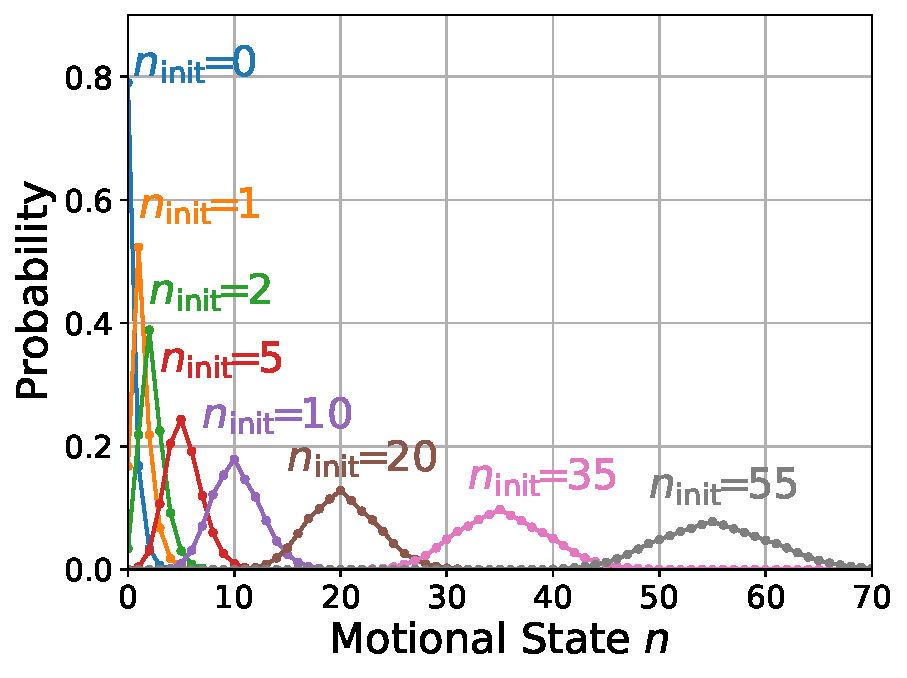
\includegraphics[width=5.4cm]{figures/rsc_op_branching.pdf}};
      }
      \visible<10->{
        \node[below] at (0.6, 3.7) {\includegraphics[width=6.3cm]{figures/rsc_sequence.pdf}};
      }
      \visible<6-8>{
        \node[below] at (0.5, 0.5) {\includegraphics[width=5.4cm]{figures/rsc_raman_rabi_1.pdf}};
      }
      \visible<7-8>{
        \draw[->,line width=1.8,>=stealth,red] (0.8, -1.0) -> (0.0, -1.8);
        \draw[->,line width=1.8,>=stealth,red] (1.4, -1.0) -> (2.8, -1.8);
        \node[red,above] at (1.1, -0.95) {Dead zone};
      }
      \visible<9-10>{
        \node[below] at (0.5, 0.5)
        {\includegraphics[width=5.4cm]{figures/rsc_raman_rabi_all.pdf}};
      }
      \visible<11->{
        \node[below,align=center] at (0.5, 0.5) {
          Axial sideband spectrum\\
          \includegraphics[width=5.4cm]{figures/rsc_spectrum_az.pdf}
        };
      }
    \end{tikzpicture}
  \end{center}
\end{frame}
\fi

\section{Molecule creation}
\subsection{Atom-atom interaction}
%% Atom-atom interaction
% So now we have achieved full quantum control on our atoms, __(>>12>>)__
% the next thing we would like is to transfer this control onto the molecules.
% But before that,
% we need to have a better understanding of the interaction between the atoms.
% This will give us information about the molecular state we want to form,
% how we can get there,
% and it will actually also help us to better prepare our atoms to form the molecules
% as you'll see later.
% It turns out that our tweezer is actually also a very good platform for such measurements.
% __(32/25:55)__
\ifSlide{interaction_shift_outline}
\begin{frame}{Outline}
  \tableofcontents[currentsection,currentsubsection]
\end{frame}
\fi

%% Scattering length
% __(>>13>>)__ The important property that we are interested in here
% is basically the scattering length between the Na and Cs atoms.
% This is a number that describes the short range interaction
% between two particles at ultracold temperature.
% The related specific properties that we are interested in includes, __(>>)__
% __(33/26:20)__

% * Binding energy of the least bound state,
% % which directly determines the scattering length to a good approximation, __(>>)__
% * Molecular potential which ultimately give rise to the bound states, __(>>)__
% * And both of these directly help us to understand the molecule better
% % when we want to create them later, __(>>)__
% * And although not directly related to what I'll focus on today,
% % this also help us to refine predictions for FB resonances
% % which is used in another one of our experiments.
% __(34/27:00)__
\ifSlide{interaction_shift_scattering_length}
\begin{frame}{Scattering length $a$}
  \begin{columns}
    \column{4.5cm}
    \begin{itemize}
    \item<2-> Binding energy
    \item<3-> Molecular potential
    \item<4-> Molecule formation
    \item<5-> Feshbach resonance\\
      $\vdots$
    \end{itemize}
    \column{6.5cm}
    \begin{tikzpicture}
      \begin{scope}[scale=0.65]
        \draw[->,>=stealth,line width=1.2] (0, 0) -- (0, 8);
        \node[above,rotate=90] at (0, 4) {Energy};
        \draw[->,>=stealth,line width=1.2] (0, 0) -- (8, 0);
        \node[below] at (4, -0.5) {Internuclear Distance};

        \draw[dashed] (1.0269 - 0.25, 2.5) -- (7 - 0.25, 2.5);
        \draw (1.0793 - 0.25, -0.4631 + 2.5) -- (4.5 - 0.25, -0.4631 + 2.5);

        \draw[line width=1.1]
        plot[samples=200,domain=0.8:7,variable=\x]
        ({\x - 0.25}, {6.8*\x^(-3.4)-6.5*\x^(-1.7) + 2.5});

        \mytweezer.drawNaAtom(5.55, 2.7, 0.12)
        \mytweezer.drawCsAtom(6.05, 2.7, 0.10)

        \mytweezer.drawNaAtom(2.08, 2.15, 0.12)
        \mytweezer.drawCsAtom(2.25, 2.15, 0.10)

        \draw[->,>=stealth,cyan!50!blue,line width=0.8] (5.4, 2.7) -- ++(-3.5, 0)
        arc (270:90:0.2) -- ++(2.5, 0);
      \end{scope}
    \end{tikzpicture}
  \end{columns}
\end{frame}
\fi

%% Interaction shift
% We measure the scattering length using interaction shift and it works like this. __(>>14>>)__
% If we successfully loaded two atoms in the tweezer,
% their energy levels will be shifted due to the interaction between them
% compared to if we only have one loaded.
% Now this cannot be directly compared to the single atom case as showned here
% since we can't really drive an atom in and out out of the tweezer
% in a controlled manner. __(>>)__
% So instead, we rely on the fact that this interaction is in general state dependent.
% If we drive the atoms from one spin combinantion to a different one,
% say with a Raman transition or a microwave,
% we should be able to see a shift in the resonance frequency,
% corresponding to the difference of the interaction energy
% between the initial and final spin states.
% This way of measuring the scattering length
% is similar to the experiement done in optical lattices in MOTT insulator phase
% but the anisotropy of the trap causes some difference which you'll see shortly.
% __(35/28:10)__

% So we did the measurement. __(>>)__
% Here's the resonance when only Cs atom is loaded in the trap.
% Compared to this, if we measured an interaction shifted peak on the right,
% it would suggest that the final state has a higher energy
% or a more repulsive interaction than the initial state,
% whereas a peak on the left would mean a more attractive final state.
% __(36/28:40)__

% Now when we added the Na atom, __(>>)__
% instead of seeing one peak, we actually saw three peaks.
% Well, the center one is easy, our state preparation isn't perfect
% and in this case only 60-70% of the atoms are in the ground state
% and the hot atoms has lower density and much lower shift
% so it appears closer to the bare resonance.
% We were very confused by the other two peaks though.
% Since not only do we have more than one interaction shifted peaks,
% it seems that they don't even agree on the sign of the interaction.
% __(37/29:25)__

% So we were puzzled by our data for a while,
% until we realized that the interaction shift that we've observed here
% is actually very similar to the axial trapping frequency.
% This means that the interaction will be strong enough to mix motional states
% and we can't simply treat it as pertubation anymore. __(>>)__
% In order to accurately calculate this,
% we have to go back to the full Hamiltonian shown here
% which has the term for Na, Cs and their interaction
% and we'll approximate the interaction by a contact potential
% that is proportional to the scattering length.
% __(38/)__

% This is not a easy problem to solve of course
% and it actually helps to do a coordinate transformation. __(>>)__
% Instead of using the Na and Cs coordinates,
% the center of mass and relative coordinates are much more natural choices
% to discribe the interaction,
% for example, like what we want to calculate here
% and also when talking about molecule formation later.
% The transformation itself is actually the same one in freshman classical mechanics
% and after that the Hamiltonian now looks like this,
% with a center of mass part, as a simple harmonic oscillator,
% a relative part, which is the a harominic oscillator plus the interaction,
% and a mixing part caused by the difference in the Na and Cs trapping frequencies.
% __(39/31:10)__

% The solution to the first part is very easy and it turns out that the second part,
% harmonic oscillator with contact interaction, is also important enough
% that people have worked out analytic solutions for it as well,
% so the only part that we need to do ourselves is the mixing term
% which is much more well behaved compared to the contact interaction
% and it can be solved numerically fairly easily.
% So we did it __(>>)__ and the energy levels,
% plotted as functions of the scattering length looks like this.
% Each spin state, with its specific scattering length
% corresponds to a vertical slice on this plot
% and driving transitions between them corresponds to moving horizontally.
% Different curves corresponds to atoms in a different motional states,
% which may have center of mass or relative motion excitation or a mixture of the two.
% __(40/32:20)__

% It is now much easier to understand our signal. __(>>)__
% It turns out that in this case, our initial state has a very small scattering length
% and our final state has a large and negative one.
% The peak on the left seems to be actually the "normal" interaction shifted signal
% where the atoms remained in the motional ground state of the system after the transition.
% The signal on the right actually corresponds to the atoms acquring some motional energy
% in additional to the interaction energy,
% which puts it on the wrong side of the unshifted peak.
% __(41/32:55)__

% We've also measured the shift for other spin state combinations
% and this explanation works out as well. __(>>)__
% Here I'm showing a case where the normal signal
% and the one with motional excitation appears on the same side
% instead of two different sides.
% __(42/33:25)__

% Combining this with some of our other measurements,
% we can now fit the data using our model
% and calculate the scattering length for the other spin state combinations __(>>)__
% and you can see the results here.
% __(43/33:40)__

% While this is cool, of course we did this measurement not just to show how nice it is
% to use optical tweezer to trap and control atoms or watch them interact,
% we did this also to help us making the molecules.
% For that, the numbers shown here are used, as I said earlier,
% to help us find some of the bound states and FB resonance.
% __(44/34:10)__

% I also want to point out that the 3,3+2,2 combination has a very strong interaction.
% This suggests that the atomic wavefunction is strongly affected by the molecular potential
% which should enhance the coupling from this state to the molecular state. __(>>)__
% Indeed, if we look at the wavefunction for these spin states,
% we'll see that the 3322 one has significantly more wavefunction component
% at short distance closer to and inside the molecular potential,
% making it the most "molecule like" atomic state.
% For this reason, we select this state to form our molecule as you'll see in the next part.
% __(45/35:00)__

% Another advantage for selecting this state is that
% this actually also help us preparing the atomic state itself. __(>>)__
% If we have another look at the interaction shift signal here,
% we said that the peak on the right corresponds to the atom acquiring some motional excitation
% whereas the left one corresponds to the atom remaining in the ground state.
% In another word, if we drive on the left peak, __(>>)__
% we can actually select out only the ground state atoms.
% This allow us to reduce the background of our signal
% and to be able to work even when our cooling isn't perfect.
% This improves the robustness and signal to noise of our experiment.
% __(46/35:45)__
\ifSlide{interaction_shift_result}
\begin{frame}{Interaction shift}
  \vspace{-0.8cm}
  \begin{tikzpicture}
    \draw[white,opacity=0] (-6, -4.5) rectangle (6, 4.5);
    % Raman sequence
    \visible<-4>{
      \begin{scope}[shift={(-3, 0)}]
        \begin{scope}[shift={(-1.79, 0.78)}]
          \draw[dashed,gray,line width=0.8] (0.35, {0.35^2 * 3.5}) -- (3.4, {0.35^2 * 3.5})
          coordinate (Upper Energy 1);
          \draw[line width=1.5] plot[domain={-0.65:0.65},smooth,variable=\x]
          ({\x}, {(\x)^2 * 3.5});
          \draw[line width=0.8] (-0.35, {0.35^2 * 3.5}) -- (0.35, {0.35^2 * 3.5});
          \draw[line width=0.8,-{Latex[length=1.2mm,width=1.2mm]}]
          (0, {0.35^2 * 3.5 - 0.25}) -- (0, {0.35^2 * 3.5 + 0.3});
          \coordinate (Upper Atom 1) at (0, {0.35^2 * 3.5});
          \mytweezer.drawCsAtom(0, {0.35^2 * 3.5}, 0.14)
          \node[above] at (0, 1.48) {\small Single Atom};
        \end{scope}
        \begin{scope}[shift={(0.4, 1.35)}]
          \draw[dashed,gray,line width=0.8] (0.35, {0.35^2 * 3.5}) -- (1.21, {0.35^2 * 3.5})
          coordinate (Upper Energy 2);
          \draw[line width=1.5] plot[domain={-0.65:0.65},smooth,variable=\x]
          ({\x}, {(\x)^2 * 3.5});
          \draw[line width=0.8] (-0.35, {0.35^2 * 3.5}) -- (0.35, {0.35^2 * 3.5});
          \draw[line width=0.8,-{Latex[length=1.2mm,width=1.2mm]}]
          (-0.14, {0.35^2 * 3.5 - 0.25}) -- (-0.14, {0.35^2 * 3.5 + 0.3});
          \coordinate (Upper Atom 2) at (-0.14, {0.35^2 * 3.5});
          \mytweezer.drawCsAtom(-0.14, {0.35^2 * 3.5}, 0.14)
          \draw[line width=0.8,-{Latex[length=1.2mm,width=1.2mm]}]
          (0.16, {0.35^2 * 3.5 - 0.25}) -- (0.16, {0.35^2 * 3.5 + 0.3});
          \mytweezer.drawNaAtom(0.16, {0.35^2 * 3.5}, 0.18)
          \node[above] at (0, 1.48) {\small Two Atoms};
        \end{scope}
        \path (Upper Energy 1) -- node[right] {$V_{\rm int}$} (Upper Energy 2);
        \draw[latex-latex,line width=0.8] ($(Upper Energy 1) - (0.2, 0)$)
        -- ($(Upper Energy 2) - (0.2, 0)$);

        \visible<2->{
          \begin{scope}[shift={(-0.99, -1)}]
            \draw[dashed,gray,line width=0.8] (0.35, {0.35^2 * 3.5}) -- (3.5, {0.35^2 * 3.5})
            coordinate (Lower Energy 1);
            \draw[line width=1.5] plot[domain={-0.65:0.65},smooth,variable=\x]
            ({\x}, {(\x)^2 * 3.5});
            \draw[line width=0.8] (-0.35, {0.35^2 * 3.5}) -- (0.35, {0.35^2 * 3.5});
            \draw[line width=0.8,-{Latex[length=1.2mm,width=1.2mm]}]
            (0, {0.35^2 * 3.5 + 0.25}) -- (0, {0.35^2 * 3.5 - 0.3});
            \coordinate (Lower Atom 1) at (0, {0.35^2 * 3.5});
            \mytweezer.drawCsAtom(0, {0.35^2 * 3.5}, 0.14)
          \end{scope}
          \begin{scope}[shift={(1.5, -1.5)}]
            \draw[dashed,gray,line width=0.8] (0.35, {0.35^2 * 3.5}) -- (1.01, {0.35^2 * 3.5})
            coordinate (Lower Energy 2);
            \draw[line width=1.5] plot[domain={-0.65:0.65},smooth,variable=\x]
            ({\x}, {(\x)^2 * 3.5});
            \draw[line width=0.8] (-0.35, {0.35^2 * 3.5}) -- (0.35, {0.35^2 * 3.5});
            \draw[line width=0.8,-{Latex[length=1.2mm,width=1.2mm]}]
            (-0.14, {0.35^2 * 3.5 + 0.25}) -- (-0.14, {0.35^2 * 3.5 - 0.3});
            \coordinate (Lower Atom 2) at (-0.14, {0.35^2 * 3.5});
            \mytweezer.drawCsAtom(-0.14, {0.35^2 * 3.5}, 0.14)
            \draw[line width=0.8,-{Latex[length=1.2mm,width=1.2mm]}]
            (0.16, {0.35^2 * 3.5 - 0.25}) -- (0.16, {0.35^2 * 3.5 + 0.3});
            \mytweezer.drawNaAtom(0.16, {0.35^2 * 3.5}, 0.18)
          \end{scope}
          \path (Lower Energy 1) -- node[right] {$V_{\rm int}^*$} (Lower Energy 2);
          \draw[latex-latex,line width=0.8] ($(Lower Energy 1) - (0.2, 0)$)
          -- ($(Lower Energy 2) - (0.2, 0)$);

          \draw[latex-latex,red,line width=0.9,shorten <=0.12cm,shorten >=0.12cm]
          (Upper Atom 1) -- (Lower Atom 1);
          \draw[latex-latex,red,line width=0.9,shorten <=0.12cm,shorten >=0.12cm]
          (Upper Atom 2) -- node[right] {\Large $\Omega_{\rm Raman}$} (Lower Atom 2);
        }
      \end{scope}
    }
    % Data 1
    \visible<3-9>{
      \draw[->,>=stealth,line width=1,red!50!black]
      (3.63, 1.4) -- node[above] {\small Repulsive} ++(1.8, 0);
      \draw[->,>=stealth,line width=1,green!50!black]
      (3.5, 1.4) -- node[above=0.07cm] {\small Attractive} ++(-1.8, 0);
    }
    \visible<3>{\node at (3.2, -0.4) {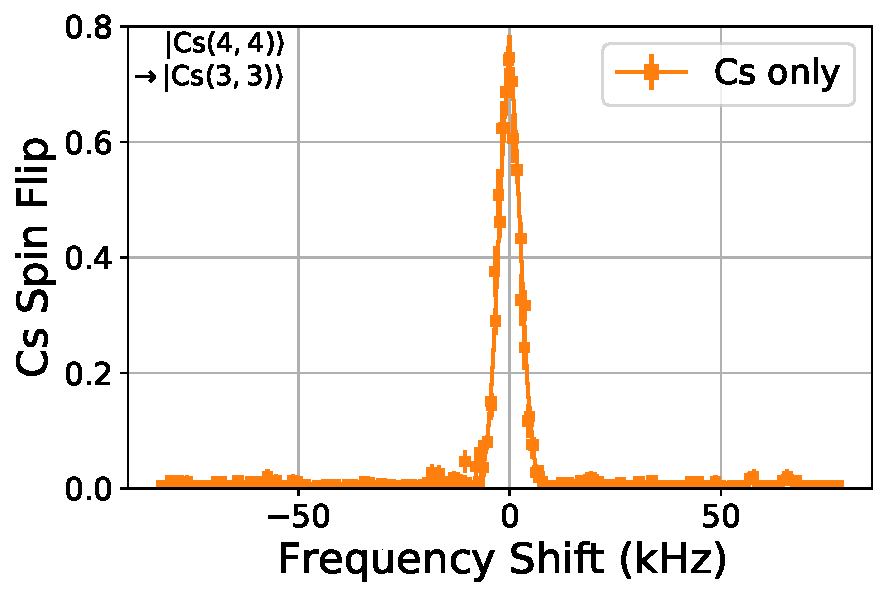
\includegraphics[width=5cm]{
          figures/interaction_shift_spectrum_42_32_cs.pdf}};}
    \visible<4-8>{\node at (3.2, -0.4) {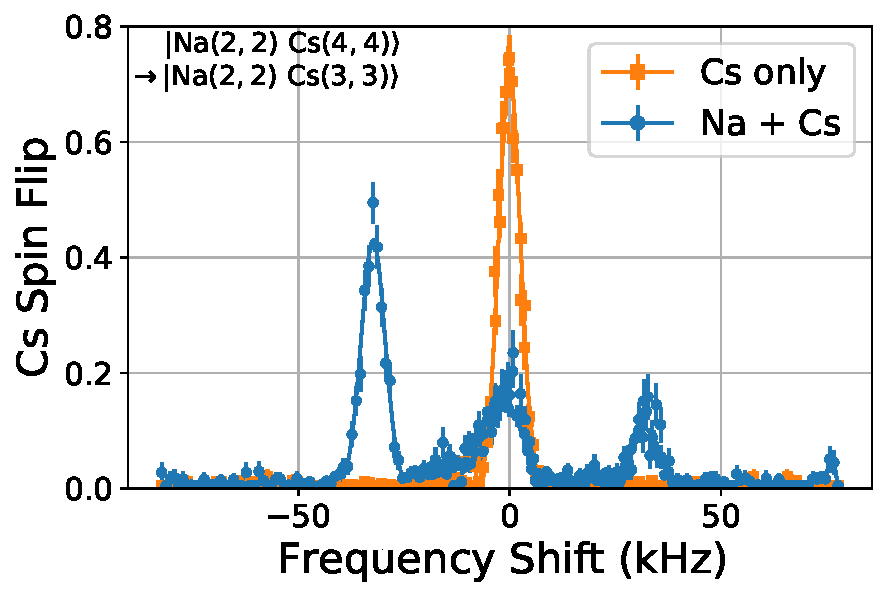
\includegraphics[width=5cm]{
          figures/interaction_shift_spectrum_42_32_nostate.pdf}};}
    \visible<9>{\node at (3.2, -0.4) {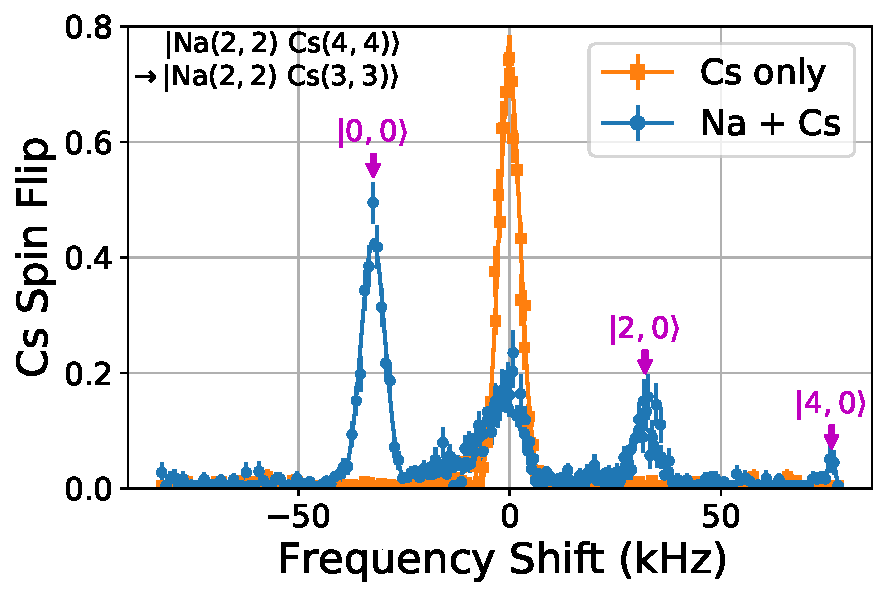
\includegraphics[width=5cm]{
          figures/interaction_shift_spectrum_42_32.pdf}};}
    \visible<10->{
      \node at (3.2, -0.4) {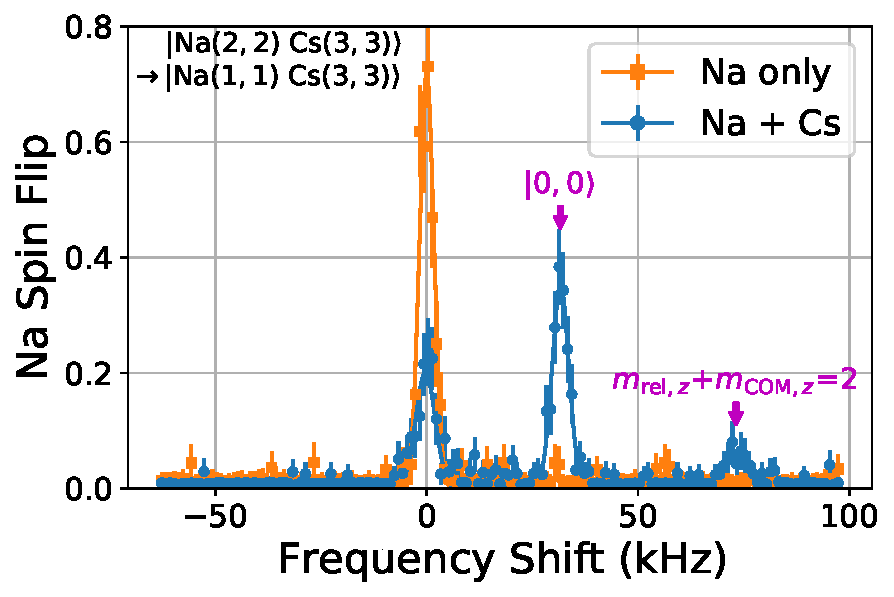
\includegraphics[width=5cm]{
          figures/interaction_shift_spectrum_32_31.pdf}};
      \draw[->,>=stealth,line width=1,red!50!black]
      (3.13, 1.4) -- node[above] {\small Repulsive} ++(1.8, 0);
      \draw[->,>=stealth,line width=1,green!50!black]
      (3.0, 1.4) -- node[above=0.07cm] {\small Attractive} ++(-1.5, 0);
    }

    % Equations
    \visible<5-7>{
      \node[below right,align=left] at (-4.9, 3.8)
      {\footnotesize $\displaystyle H=\!\!\sum_{i=x,y,z}(\frac{m_{1}\omega_{1,i}^2x_{1,i}^2}{2}+\frac{p_{1,i}^2}{2m_{1}})\ +\!\sum_{i=x,y,z}(\frac{m_{2}\omega_{2,i}^2x_{2,i}^2}{2}+\frac{p_{2,i}^2}{2m_{2}})+V_{\rm int}(\vec r_1-\vec r_2)$};
      \draw[decoration={brace,mirror,amplitude=10pt},decorate,line width=1]
      (-4.15,2.8) -- node[below=10pt] {\small Na} (-1.15,2.8);
      \draw[decoration={brace,mirror,amplitude=10pt},decorate,line width=1]
      (-0.5,2.8) -- node[below=10pt] {\small Cs} (2.5,2.8);
      \draw[decoration={brace,mirror,amplitude=8pt},decorate,line width=1]
      (3.05,2.8) -- node[below=10pt] {\small Interaction} (4.55,2.8);
    }
    \visible<6-7>{
      \begin{scope}[shift={(-3.8, 0.7)}]
        \draw[line width=1] plot[domain={-0.9:0.9},smooth,variable=\x]
        ({\x * 0.8}, {(\x)^2 * 1.5});
        \mytweezer.drawNaAtom(0.05, 0.4, 0.16)
        \draw[->,atomorange,line width=0.8] (-0.3, 0.6) -- (0.3, 0.6);
        \node[atomorange] at (0.6, 0) {\small Na};
      \end{scope}

      \begin{scope}[shift={(-2.5, 1.3075)}]
        \draw[line width=1] (-0.3, 0) -- (0.3, 0);
        \draw[line width=1] (0, -0.3) -- (0, 0.3);
      \end{scope}

      \begin{scope}[shift={(-1.2, 0.7)}]
        \draw[line width=1] plot[domain={-0.9:0.9},smooth,variable=\x]
        ({\x * 0.8}, {(\x)^2 * 1.5});
        \mytweezer.drawCsAtom(-0.05, 0.3, 0.12)
        \draw[->,blue,line width=0.8] (0.3, 0.5) -- (-0.3, 0.5);
        \node[blue] at (0.6, 0) {\small Cs};
      \end{scope}

      \draw[->,line width=2.5] (-2.5, 0.55) -- (-2.5, -0.885);

      \begin{scope}[shift={(-3.8, -2.3)}]
        \draw[line width=1] plot[domain={-0.9:0.9},smooth,variable=\x]
        ({\x * 0.8}, {(\x)^2 * 1.5});
        \mytweezer.drawNaAtom(0.15, 0.4, 0.16)
        \mytweezer.drawCsAtom(-0.15, 0.4, 0.12)
        \draw[->,atomorange,line width=0.8] (-0.1, 0.6) -- (0.4, 0.6);
        \draw[->,blue,line width=0.8] (-0.4, 0.7) -- (0.1, 0.7);
        \node[align=left,
        execute at begin node=\setlength{\baselineskip}{9pt}]
        at (-0.95, 0.25) {\small Center\\\small of mass};
      \end{scope}

      \begin{scope}[shift={(-2.5, -1.5925)}]
        \draw[line width=1] (-0.3, 0) -- (0.3, 0);
        \draw[line width=1] (0, -0.3) -- (0, 0.3);
      \end{scope}

      \begin{scope}[shift={(-1.2, -2.3)}]
        \draw[line width=1] plot[domain={-0.9:0.9},smooth,variable=\x]
        ({\x * 0.8}, {(\x)^2 * 1.5});
        \mytweezer.drawNaAtom(0.2, 0.5, 0.16)
        \mytweezer.drawCsAtom(-0.25, 0.5, 0.12)
        \draw[->,atomorange,line width=0.8] (0, 0.7) -- (0.47, 0.7);
        \draw[->,blue,line width=0.8] (-0.08, 0.7) -- (-0.45, 0.7);
        \node at (1, 0.15) {\small Relative};
      \end{scope}
    }
    \visible<7->{
      \node[above right,align=left] at (-6, -4.5)
      {\footnotesize $\displaystyle H=\!\!\sum_{i=x,y,z}(\frac{M\Omega_{i}^2X_{i}^2}{2}+\frac{P_{i}^2}{2M})\ +\!\sum_{i=x,y,z}(\frac{\mu\omega_{\mathrm{R},i}^2x_{\mathrm{R},i}^2}{2}+\frac{p_{\mathrm{R},i}^2}{2\mu})+V_{\rm int}(\vec r_\mathrm{R})\ +\!\sum_{i=x,y,z}\mu(\omega_{1,i}^2 - \omega_{2,i}^2)X_ix_{\mathrm{R},i}$};
      \draw[decoration={brace,amplitude=10pt},decorate,line width=1]
      (-5.25,-3.5) -- node[above=10pt] {\small Center of mass} (-2.5,-3.5);
      \draw[decoration={brace,amplitude=10pt},decorate,line width=1]
      (-1.9,-3.5) -- node[above=10pt] {\small Relative} (2.4,-3.5);
      \draw[decoration={brace,amplitude=10pt},decorate,line width=1]
      (3,-3.5) -- node[above=10pt] {\small Mixing} (5.9,-3.5);
    }
    \visible<8>{
      \node at (-2.6, 0.5) {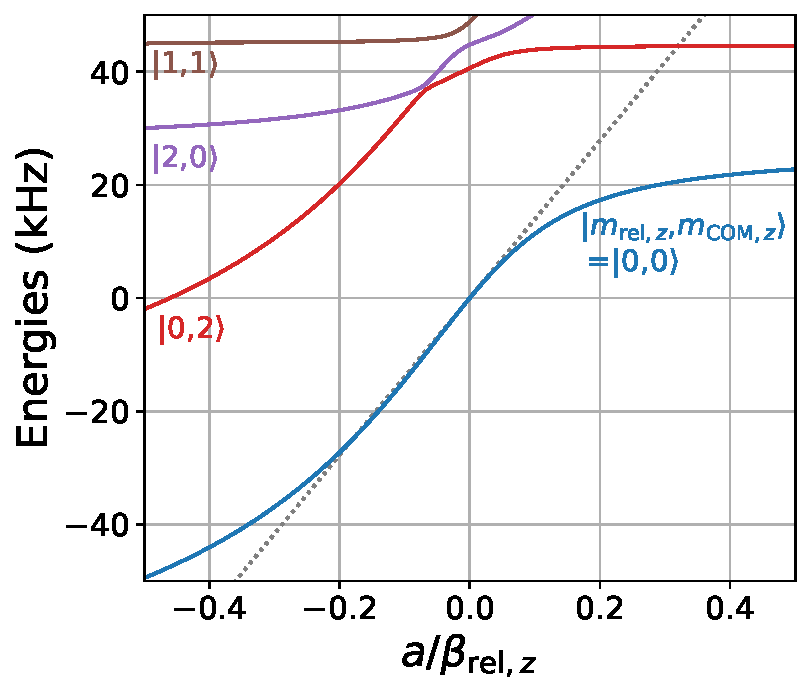
\includegraphics[width=6cm]{
          figures/interaction_shift_energies.pdf}};
    }
    \visible<9>{
      \node at (-2.6, 0.5) {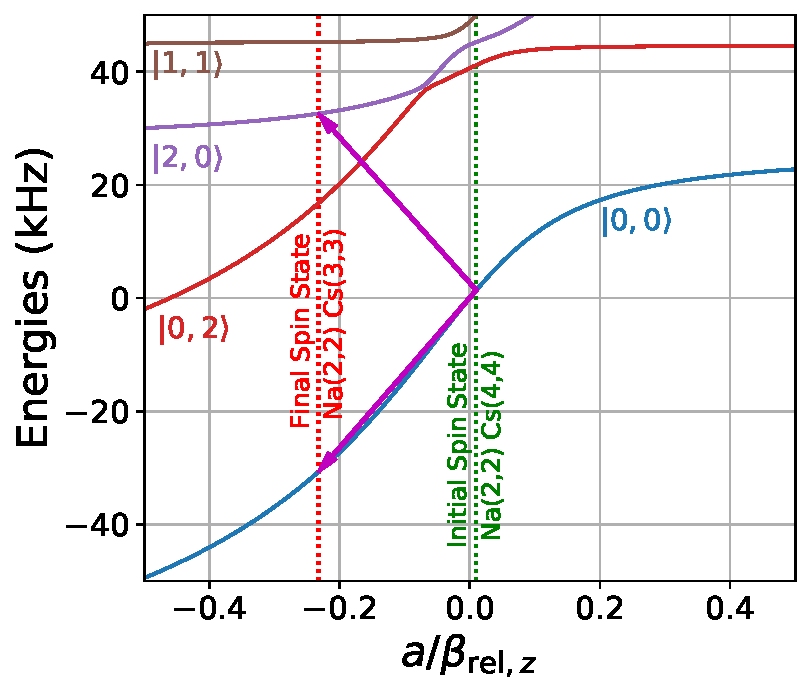
\includegraphics[width=6cm]{
          figures/interaction_shift_energies_42_32.pdf}};
    }
    \visible<10->{
      \node at (-2.6, 0.5) {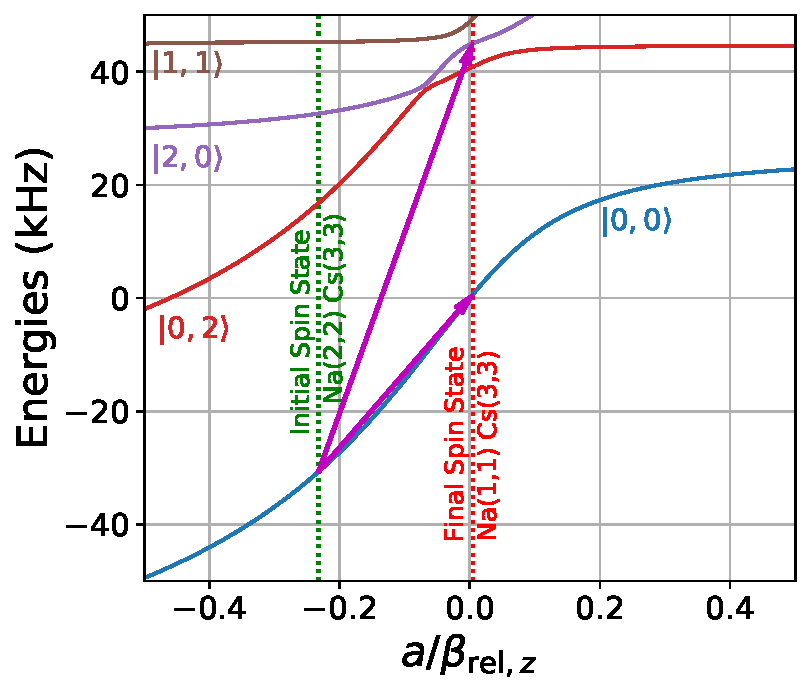
\includegraphics[width=6cm]{
          figures/interaction_shift_energies_32_31.pdf}};
    }
    \visible<11->{
      \fill[white,opacity=0.95] (-6, -4.5) rectangle (6, 3.5);
      \node[align=center] at (0, 2.1)
      {Combined with binding energy measurement on Na(2,2) Cs(4,4)\\
        \\
        \begin{tabular}{|c|c|}
          \hline
          Spin state ($F,m_F$)&Scattering length (a.u.)\\\hline
          Na(2,2) Cs(4,4)&30.36\\\hline
          Na(2,2) Cs(3,3)&-693.8\\\hline
          Na(1,1) Cs(3,3)&13.19\\\hline
        \end{tabular}};
    }
    \visible<12->{
      \draw[->,>=stealth,line width=1,color=red!50!black] (0.8, 1.45) -- (-1.5, 0.3)
      node[below] {Enhanced coupling to molecular state!};
      \node[below] at (-3, -0.3) {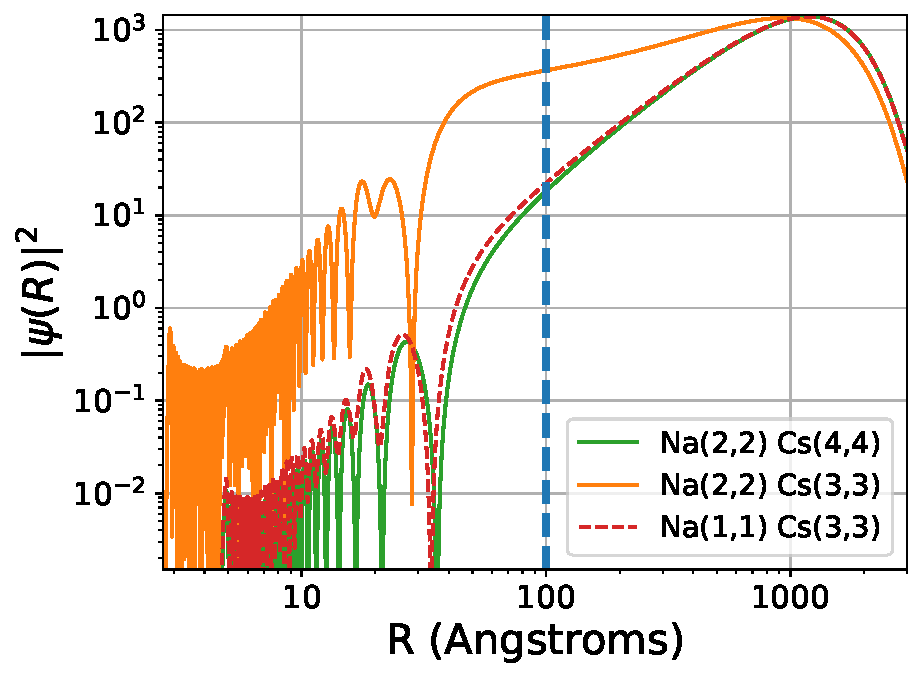
\includegraphics[width=5.5cm]{
          figures/interaction_shift_atomic_wavefunction.pdf}};
    }
    \visible<13->{
      \node[below] at (3, -0.8) {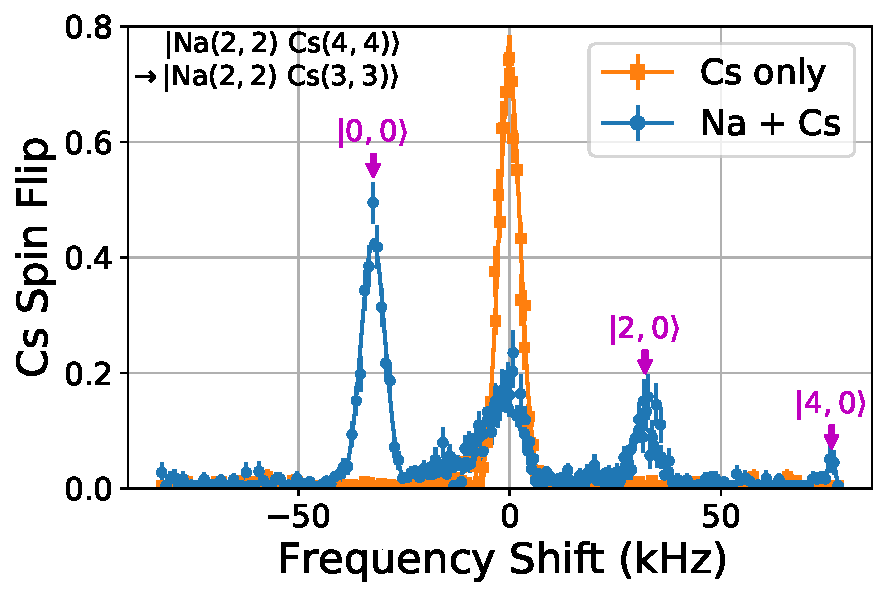
\includegraphics[width=5cm]{
          figures/interaction_shift_spectrum_42_32.pdf}};
    }
    \visible<14->{
      \node[below,blue] (GroundStateText) at (3.0, -0.3) {Ground State Only};
      \draw[->,>=stealth,blue,line width=2] (GroundStateText) -- (2.6, -2.0);
    }
  \end{tikzpicture}
\end{frame}
\fi

\subsection{Coherent optical transfer}
%% Optical molecule creation
% So now we've prepared the states of the atoms and
% we've measured the properties of their interaction. __(>>15>>)__
% I'll now talk about how we make the molecules while maintaining the quantum control.
% __(47/36:00)__
\ifSlide{raman_transfer_outline}
\begin{frame}{Outline}
  \tableofcontents[currentsection,currentsubsection]
\end{frame}
\fi

%% Size mismatch
% So just to remind you, __(>>16>>)__ here's a summary of our control of the atom,
% needed before we form the molecule.
% After we merge the two atoms into the same tweezer,
% the two atoms are about as closed to each other as they can be from the confinement.
% Nevertheless, __(>>)__ comparing to the molecule we want to make,
% it is still a few hundred times bigger.
% This massive size mismatch is really the biggest challange
% for anyone who want to create molecules coherently from atoms. ...
% __(48/36:40)__
\ifSlide{raman_transfer_size}
\begin{frame}{}
  \begin{center}
    \begin{tikzpicture}
      \node[below,align=center] at (1.75, 4)
      {\hspace{0.5cm}\usebeamerfont{frametitle}\usebeamercolor[fg]{frametitle}{Loading}\\
        \includegraphics[width=3cm]{figures/overview_single_atom.png}};
      \node[above,align=center] at (2, 0.36)
      {\usebeamercolor[fg]{frametitle}{\tiny{NJP. 19, 023007 (2017)}}};
      \node[below,align=center] at (2.1, 0.28)
      {\usebeamerfont{frametitle}\usebeamercolor[fg]{frametitle}{Cooling}\\
        \includegraphics[width=4.2cm]{figures/rsc_spectrum_az.pdf}};
      \node[below,align=center] at (5.25, 3.5)
      {\usebeamerfont{frametitle}\usebeamercolor[fg]{frametitle}{Merging}};
      \node[above,align=center] at (2.2, -3.3)
      {\usebeamercolor[fg]{frametitle}{\tiny{\textbf{Y. Yu} et al. PRA. 97, 063423 (2018)}}};
      \node[above,align=center] at (5.4, -3.1)
      {\usebeamercolor[fg]{frametitle}{\tiny{\textbf{Y. Yu} et al. PRX. 9, 021039 (2019)}}};
      \begin{scope}[shift={(4.8, 4)}, xscale=-0.8, yscale=0.8]
        \mytweezer.drawCsTweezer(0, -3.1)
        \mytweezer.drawNaTweezer(-1, -3.1)
        \mytweezer.drawCsAtom(0.0, -3.1, 0.12)
        \mytweezer.drawNaAtom(-1.0, -3.1, 0.16)

        \mytweezer.drawCsTweezer(-1, -7.0)
        \mytweezer.drawNaAtom(-1.05, -6.87, 0.16)
        \mytweezer.drawCsAtom(-0.95, -7.13, 0.12)

        \begin{scope}[opacity=0.7]
          \draw[->,>=stealth,atomorange,line width=1.2] (-1, -3.3) -- (-1, -6.7);
          \draw[->,>=stealth,blue,domain=-3.3:-6.7,smooth,variable=\y,line width=1.2]
          plot ({atan((\y+4.7) * 5) / 170 - 0.5},{\y});
        \end{scope}
      \end{scope}
      \visible<2->{
        \begin{scope}[shift={(9.5, 2.5)}, scale=0.8]
          \draw[line width=1] plot[samples=200,domain=-2:2,variable=\x] ({\x + 0}, {(\x)^2 * 0.8 - 1.5});
          \draw[line width=2,orange!90!black]
          plot[samples=200,domain=-2:2,variable=\x] ({\x + 0}, {exp(-(\x)^2 * 1.3) - 0.988});
          \draw[line width=0.8] (0 - 0.8, -0.988) -- (0 + 0.8, -0.988);
          \draw[<->,>=stealth,line width=1] (0 - 1, 0.3) -- (0 + 1, 0.3);
          \path (0, 0.3) node[above] {$1000a_0$};
          \path (0, -1.8) node[below] {\textbf{Atom}};
        \end{scope}
        \begin{scope}[shift={(9.5, -1.5)}, scale=0.8]
          \shade[ball color=blue!90] (0, 0) circle (0.45);
          \shade[ball color=orange!90] (0.4, 0.2) circle (0.3);
          \draw[<->,>=stealth,line width=1] (-0.45, 0.4) -- (0.35, 0.8);
          \path (-0.05, 0.6) node[rotate=26.565,above=2pt] {$4a_0$};
          \path (0, -1) node[below] {\textbf{Molecule}};
        \end{scope}
      }
    \end{tikzpicture}
  \end{center}
\end{frame}
\fi

%% Two step transfer
% ... which basically necessitate a two step transfer process __(>>17>>)__.
% The more loosely bound molecular state in the middle
% reduces the size mismatch for each steps
% and will improve overall transfer efficiency. __(>>)__
% The transfer to this intermediate state is what I'll focus on in this part of the talk.
% __(49/37:00)__

% The "tranditional" choice of the intermediate state is a FB molecule. __(>>)__
% Indeed, it also works for us and **using a different apparatus
% which includes a big magnetic field coil,
% different from the one I've shown you a picture of,**
% we've recently created a single FB molecule in the optical tweezer
% and even the next step transfer to the rovibraonic ground state. __(>>)__
% However, this approach obviously rely on finding a good FB resonance
% and usually a large magentic field.
% __(50/37:35)__

% What I am going to mainly talk about today, OTOH,
% is a different approach that uses only optical transitions. __(>>)__
% By not relying on FB resonance, it is faster, more compact in setup,
% and most importantly, we hope it can be more generally apply to molecules
% that may not have a suitable FB resonance
% and only require laser cooling on the atoms themselves.
% __(51/38:10)__

% It's worth pointing out that optical transfer **has** been done previously
% on many systems __(>>)__ include this Rb2 Raman resonance shown here as well as Sr2,
% and even a previous attempt from our lab. __(>>)__
% However, it was either done incoherently, limited by scattering,
% or, in the case of Sr2, it relies on narrow line optical transitio
% n which works very well but limits the generality of the result.
% So next I'll focus on how we overcome these limitations in our experiment.
% __(52/38:50)__
\ifSlide{raman_transfer_two_step}
\begin{frame}{}
  \begin{center}
    \begin{tikzpicture}
      \begin{scope}[shift={(-1, 0)}, scale=0.9]
        \begin{scope}[shift={(-5, 3)}, scale=0.6]
          \draw[line width=1] plot[samples=200,domain=-2:2,variable=\x] ({\x + 0}, {(\x)^2 * 0.8 - 1.5});
          \draw[line width=2,orange!90!black]
          plot[samples=200,domain=-2:2,variable=\x] ({\x + 0}, {exp(-(\x)^2 * 1.3) - 0.988});
          \draw[line width=0.8] (0 - 0.8, -0.988) -- (0 + 0.8, -0.988);
          \draw[<->,>=stealth,line width=1] (0 - 1, 0.3) -- (0 + 1, 0.3);
          \path (0, 0.3) node[above] {$1000a_0$};
          \path (0, -1.8) node[below] {\small \textbf{Atom}};
        \end{scope}
        \begin{scope}[shift={(-2.2, 3)}, scale=0.6]
          \shade[ball color=blue!90] (-0.4, -0.1) circle (0.55);
          \shade[ball color=orange!90] (0.4, 0.3) circle (0.4);
          \draw[<->,>=stealth,line width=1] (-1.05, 0.4) -- (0.55, 1.2);
          \path (-0.25, 0.8) node[rotate=26.565,above=2pt] {$\approx 20\!-\!200a_0$};
          \path (0, -1.2) node[below,align=center] {\small \textbf{Weakly-Bound}\\\small \textbf{Molecule}};
        \end{scope}
        \begin{scope}[shift={(0, 3)}, scale=0.6]
          \shade[ball color=blue!90] (0, 0) circle (0.45);
          \shade[ball color=orange!90] (0.4, 0.2) circle (0.3);
          \draw[<->,>=stealth,line width=1] (-0.45, 0.4) -- (0.35, 0.8);
          \path (-0.05, 0.6) node[rotate=26.565,above=2pt] {$4a_0$};
          \path (0, -1) node[below] {\small \textbf{Molecule}};
        \end{scope}
        \visible<2->{
          \draw[line width=1, red] (-6.4, 4.35) rectangle (-0.9, 1.35);
        }
      \end{scope}
      \visible<3-4>{
        \node at (-3, 0.8) {\usebeamercolor[fg]{frametitle}{\textbf{Feshbach molecule}}};
        \node[below, align=center] at (-3.2, 0.4)
        {\includegraphics[width=6cm]{figures/raman_transfer_fb_molecules.pdf}\\
          \tiny PRL. 124, 253401 (2020)};
        \visible<4->{
          \node[below, text width=6cm, align=left] at (3, -0.3) {\begin{itemize}
            \item Requires Feshbach resonance
            \item Usually large magnetic field
            \end{itemize}
          };
        }
      }
      \visible<5->{
        \node[below, text width=6cm, align=center] at (-3.3, 1)
        {{\usebeamercolor[fg]{frametitle}{\textbf{Optical transfer}}}\\
          \begin{itemize}
          \item More general
          \item Faster
          \end{itemize}
        };
      }
      \visible<6->{
        \node[below, text width=6cm, align=left] at (3.1, 4)
        {
          {\usebeamercolor[fg]{frametitle}{Previous results}}\\
          {\footnotesize $\mathrm{Rb_2}$}
          {\tiny \usebeamercolor[fg]{frametitle}{Science 287, 1016 (2000)}}\\
          \phantom{{\footnotesize $\mathrm{Rb_2}$}}
          {\tiny \usebeamercolor[fg]{frametitle}{PRL. 93, 073002 (2004)}}\\
          \includegraphics[width=3.5cm]{figures/raman_transfer_rb2.png}\\
          {\footnotesize $\mathrm{Sr_2}$}
          {\usebeamercolor[fg]{frametitle}{\tiny PRL. 109, 115302 (2012)}}\\
          {\footnotesize $\mathrm{NaCs}$}
          {\usebeamercolor[fg]{frametitle}{\tiny \textbf{Y. Yu} et al. PRX. 9, 021039 (2019)}}\\
          \includegraphics[width=3.5cm]{figures/raman_transfer_old.pdf}
        };
      }
      \visible<7->{
        \node[below, text width=6cm, align=center] at (-3.3, -1.3)
        {
          {\usebeamercolor[fg]{frametitle}{Limitations so far}}\\
          \begin{itemize}
          \item Incoherent due to scattering
          \item Rely on narrow line optical transition
          \end{itemize}
        };
      }
    \end{tikzpicture}
  \end{center}
\end{frame}
\fi

%% Raman scheme
% The scheme we use is actually very simple. __(>>18>>)__
% We simply drive a Raman transition from the atomic state to the molecular state,
% detuned from some excited molecular state.
% __(53/39:10)__

% Since one of the major challenges is the mismatch of the wavefunction sizes,
% it makes sense to pick molecular states that are as "big" as possible,
% in another word, ones that are closed to the dissociation threshold
% or even the first bound state. __(>>)__
% Indeed, this is what all previous attempts use
% which leads to a fairly strong Raman transition.
% __(54/)__

% But these states are also very closely spaced, and in case of the excited state,
% have smaller detuning from other molecular state and the atomic state
% causing faster scattering,
% which ultimately limits the coherence as I metioned previously. __(>>)__
% If we instead use an excited state that is more deeply bound.
% Even though the Raman coupling is reduced,
% we can now stay further away from all the other excited states
% to surpress the scattering without worrying about hitting something else.
% __(55/40:30)__

% It is certainly not obvious if the deeply bound state costs too much
% in the Raman coupling compared to the scattering reduction.
% And that's why we did a calculation to compare the two. __(>>)__
% __(56/40:45)__

% From the top plot,
% you can easily see that the Raman Rabi frequency is indeed higher overall
% for the near threshold state shown in orange,
% compared to the deeply bound intermediate state shown in blue.
% However, if we now look at the bottom plot,
% the Rabi frequency to scattering ratio can reach much higher for the deeply bound state
% when a larger detuning is used, which corresponding to a better efficiency.
% You can also clearly see that in general,
% there are just fewer states around the blue line compared to the orange one.
% __(57/41:30)__
\ifSlide{raman_transfer_state}
\begin{frame}[t]{}
  \begin{adjustwidth}{-0.35cm}{-0.35cm}
    \begin{center}
      \vspace{-0.2cm}
      \begin{tikzpicture}
        \fill[white,opacity=0] (-1.1, -1.5) rectangle (11.38, 7.5);
        \node[below right] at (-1.03, 7.235)
        {\usebeamercolor[fg]{frametitle}{\textbf{Raman transfer}}};
        \begin{scope}[scale=0.8]
          \draw[->,>=stealth,line width=1.2] (0, 0) -- (0, 8);
          \node[above,rotate=90] at (0, 4) {Energy};
          \draw[->,>=stealth,line width=1.2] (0, 0) -- (5.4, 0);
          \node[below] at (2.7, -0.1) {Internuclear Distance};

          \draw[cyan!85!blue] ({(1.0269 + 0.25) * 0.7}, 2.5) -- (7.25 * 0.7, 2.5);

          \draw[line width=1.1,cyan!85!blue]
          plot[samples=200,domain=0.96:7,variable=\x]
          ({(\x + 0.25) * 0.7}, {(6.8*\x^(-3.4)-6.5*\x^(-1.7)) * 1.3 + 2.5});

          \draw[line width=1.1,pyplotc5]
          plot[samples=200,domain=1:7.5,variable=\x]
          ({(\x - 0.75) * 0.7}, {(9.2*\x^(-2.5)-9.0*\x^(-1.3)) * 1.3 + 7.5});
          \node[above right,pyplotc5] at (0.55 * 0.7, 7.2) {${\rm c}^3\Sigma^+$};

          \visible<-2,4>{
            \draw[pyplotc5] ({(1.1102 - 0.75) * 0.7}, -0.69 * 1.3 + 7.5) --
            ({(6.5 - 0.75) * 0.7}, -0.69 * 1.3 + 7.5);
          }
          \visible<3->{
            \draw[pyplotc5] ({(1.4 - 0.75) * 0.7}, -1.8 * 1.3 + 7.5) --
            ({(2.5 - 0.75) * 0.7}, -1.8 * 1.3 + 7.5);
          }
          \visible<-2>{
            \draw[black!40,dashed,line width=1] ({(0.9 - 0.75) * 0.7}, -0.77 * 1.3 + 7.5) --
            ({(7 - 0.75) * 0.7}, -0.77 * 1.3 + 7.5);
          }
          \visible<3>{
            \draw[black!40,dashed,line width=1] ({(1.2 - 0.75) * 0.7}, -2 * 1.3 + 7.5) --
            ({(3 - 0.75) * 0.7}, -2 * 1.3 + 7.5);
          }
          \visible<4->{
            \draw[pyplotc1, line width=1]
            ({(1.1102 - 0.75) * 0.7 - 0.15}, -0.69 * 1.3 + 7.5 - 0.15) rectangle
            ({(6.5 - 0.75) * 0.7 + 0.15}, -0.69 * 1.3 + 7.5 + 0.15);
            \coordinate (ThresholdHighlight)
            at ({(6.5 - 0.75) * 0.7 + 0.25}, -0.69 * 1.3 + 7.5 - 0.08);
            \draw[pyplotc0, line width=1]
            ({(1.4 - 0.75) * 0.7 - 0.15}, -1.8 * 1.3 + 7.5 - 0.15) rectangle
            ({(2.5 - 0.75) * 0.7 + 0.15}, -1.8 * 1.3 + 7.5 + 0.15);
            \coordinate (DeepHighlight)
            at ({(2.5 - 0.75) * 0.7 + 0.25}, -1.8 * 1.3 + 7.5);
          }

          \mytweezer.drawNaAtom(6.50 * 0.7, 2.6, 0.12)
          \mytweezer.drawCsAtom(7.10 * 0.7, 2.6, 0.10)

          \draw[cyan!85!blue] ({(1.0793 + 0.25) * 0.7}, -0.28 * 1.3 + 2.5)
          -- ({(6 + 0.25) * 0.7}, -0.28 * 1.3 + 2.5);
          \draw[line width=1] (3.98 * 0.7, -0.19  * 1.3 + 2.5)
          -- (4.35 * 0.7, -0.19  * 1.3 + 2.5);
          \mytweezer.drawNaAtom(3.98 * 0.7, -0.19  * 1.3 + 2.5, 0.12)
          \mytweezer.drawCsAtom(4.35 * 0.7, -0.19  * 1.3 + 2.5, 0.10)

          \visible<-2>{
            \draw[->,>=stealth,blue!50!orange,line width=0.8] (6.8 * 0.7, 2.7)
            -- node[right=0.1] {$\Omega_{\rm up}$} ({(3.5 - 0.75) * 0.7}, -0.8 * 1.3 + 7.5);
            \draw[->,>=stealth,green!80!black,line width=0.8]
            ({(3.45 - 0.75) * 0.7}, -0.8 * 1.3 + 7.5)
            -- node[left] {$\Omega_{\rm down}$} (4.165 * 0.7, -0.12 * 1.3 + 2.5);
          }
          \visible<3>{
            \draw[->,>=stealth,blue!50!orange,line width=0.8] (6.8 * 0.7, 2.7)
            -- node[right=0.1] {$\Omega_{\rm up}$} ({(2.8 - 0.75) * 0.7}, -2 * 1.3 + 7.5);
            \draw[->,>=stealth,green!80!black,line width=0.8]
            ({(2.75 - 0.75) * 0.7}, -2 * 1.3 + 7.5)
            -- node[left] {$\Omega_{\rm down}$} (4.165 * 0.7, -0.12 * 1.3 + 2.5);
          }
        \end{scope}
        \visible<2-3>{
          \node[below, text width=5.4cm, align=center] at (8.13, 6.8)
          {
            {\usebeamercolor[fg]{frametitle}{\textbf{Near threshold states}}}\\
            \vspace{0.2cm}
            \begin{itemize}
            \item Stronger coupling\\
              ($\Omega_{\rm up}$ and $\Omega_{\rm down}$)
            \item Closely spaced
            \item Fast scattering
            \end{itemize}
          };
        }
        \visible<3>{
          \node[below, text width=5.4cm, align=center] at (8.13, 2.7)
          {
            {\usebeamercolor[fg]{frametitle}{\textbf{Deeply bound states}}}\\
            \vspace{0.2cm}
            \begin{itemize}
            \item Weaker coupling
            \item Sparsely spaced
            \item Allow larger detuning
            \item Slower scattering
            \end{itemize}
            {\tiny \usebeamercolor[fg]{frametitle}{arXiv:1701.03121(2017)}}
          };
        }
        \visible<4>{
          \node[below] at (8.13, 7.5)
          {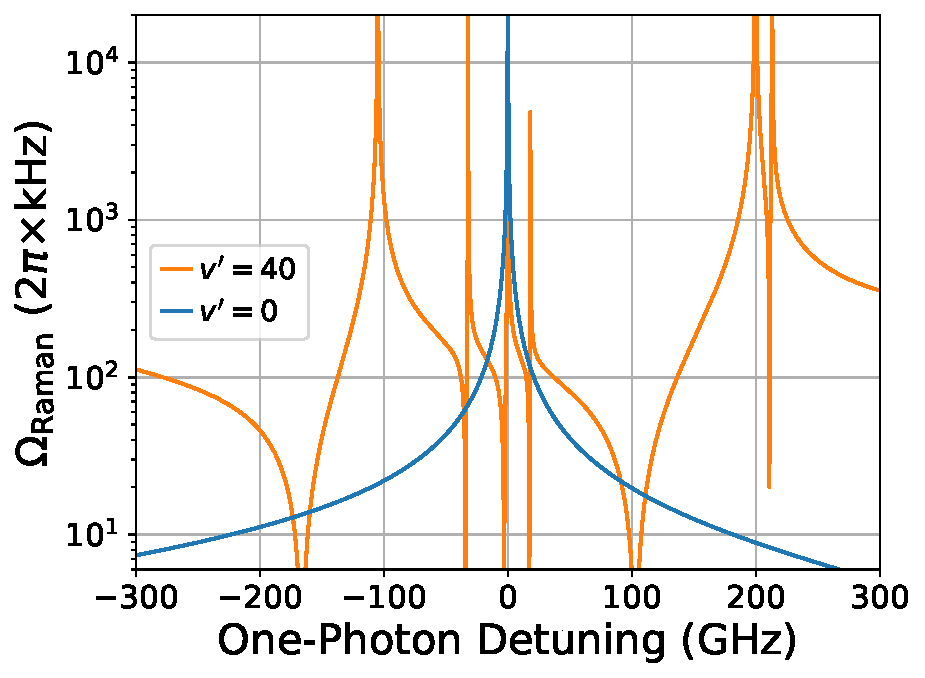
\includegraphics[width=5.4cm]{figures/raman_transfer_theory_ratio_omega.pdf}};
          \node[below] at (8.13, 3.2)
          {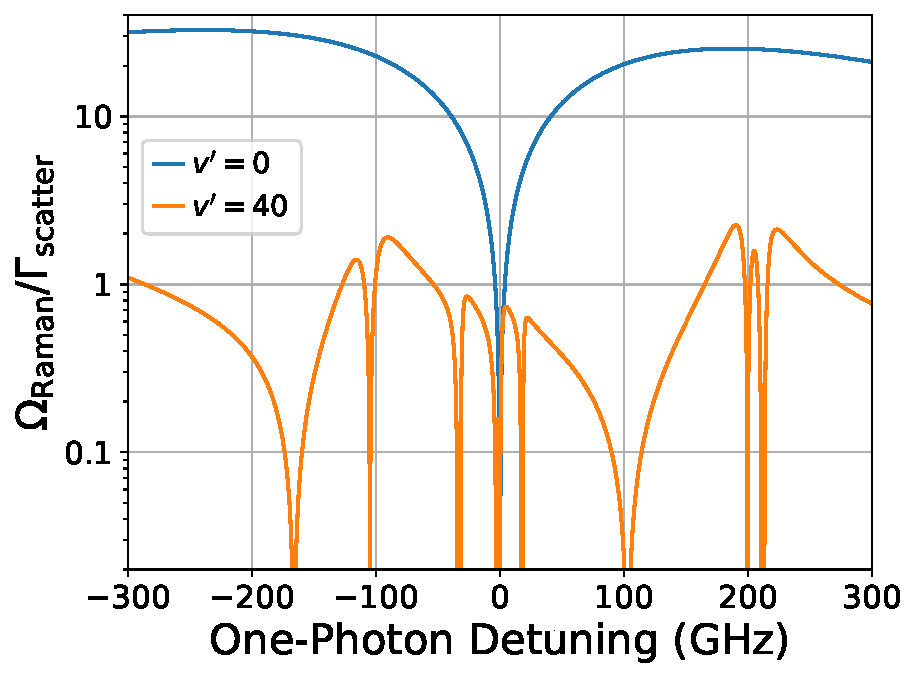
\includegraphics[width=5.4cm]{figures/raman_transfer_theory_ratio_ratio.pdf}};
        }
      \end{tikzpicture}
    \end{center}
  \end{adjustwidth}
\end{frame}
\fi

%% Experiment
% Based on the comparison, we selected the blue line,
% which corresponds to using the c3Sigma ground vibrational state,
% as the intermediate excited state,
% which we have already observed previously. __(>>19>>)__
% We initially selected an atomic state based on where we optical pump into.
% We weren't able to get a positive result from this initial state,
% including the resonance I showed on a previous slide.
% That's why we decided to change to the initial state with the biggest scattering length
% as measured in the interaction shift experiment I've just talked about
% to increase the coupling and to improve our state preparation.
% For the corresponding ground molecular state,
% the binding energy was predicted as ~771 MHz by Jeremy Hutson from Durham,
% based on our interaction shift and FB resonance measurement.
% __(58/42:30)__

% Another trick that we use is that, __(>>)__
% instead of adding another pair of beams to drive the Raman transition,
% we simply reuse our tweezer beam for that.
% We added AOMs to our tweezer beam path so that
% we can add a second frequency to our tweezer with controllable detuning.
% This allow us to take advantage of the high intensity of the tweezer
% to achieve a high Raman Rabi frequency so that we can do the transfer faster
% and beats other noise sources like magnetic field fluctuations.
% This also minimizes the number of beams we shine on the atom
% and reduce the total scattering rate from them.
% __(59/43:20)__

% Thanks to the prediction, __(>>)__ it didn't take too long for us to find the resonance,
% which was only 1-2MHz off.
% __(60/43:35)__

% But what's more important, and different from all previous spectra, __(>>)__
% is the FWHM of 8.4 kHz.
% It is very closed to the Fourier limited linewidth for the 0.1 ms pulse time we use,
% suggesting that we are already in the coherent regime.
% __(61/43:55)__

% So next, naturally, we switched to scanning the time on resonance. __(>>)__
% And sure enough we see a revival in our signal,
% which is the evidence that we can drive the atoms to molecule and then back coherently.
% Shown here is one of the typical Rabi flopping we get.
% This is the first time coherent optical transfer has been done
% without using a narrow optical transition
% and we believe it can be applied to many other systems.
% __(62/44:30)__

% The contrast is obviously not 100%, __(>>)__
% but this actually correspond to more than 60% of initial ground state atom,
% here, being transfered into the molecular state.
% You can also see it in this plot of the molecule population
% as a function of the time and detuning calculated based on the experiment results. __(>>)__
% From the design of our transfer scheme,
% all molecules we made are in a single spin state
% with 50% or even more of them in the ground motional state.
% __(63/45:10)__

% We did a lot of investigation on the difference between the theory prediction
% and the experimental observation. __(>>)__
% And we concluded that the efficiency was limited by significant scattering
% from unaccounted sources.
% This shortens the molecular lifetime which we measured here
% to be about 10 times shorter than what we expect.
% I'll save you from all the measurements we did,
% but to summarize we have identified two potential sources of extra scattering.
% __(64/45:45)__
\ifSlide{raman_transfer_result}
\begin{frame}[t]{}
  \begin{adjustwidth}{-0.35cm}{-0.35cm}
    \begin{center}
      \vspace{-0.2cm}
      \begin{tikzpicture}
        \fill[white,shift={(-5.5, -3.5)},opacity=0] (-1.1, -1.5) rectangle (11.38, 7.5);
        \node[below right,shift={(-5.5, -3.5)}] at (-1.03, 7.235)
        {\usebeamercolor[fg]{frametitle}{\textbf{Experiment}}};
        \visible<-5>{
          \begin{scope}[shift={(-5.5, -3.5)}, scale=0.8]
            \draw[->,>=stealth,line width=1.2] (0, 0) -- (0, 8);
            \node[above,rotate=90] at (0, 4) {Energy};
            \draw[->,>=stealth,line width=1.2] (0, 0) -- (5.4, 0);
            \node[below] at (2.7, -0.1) {Internuclear Distance};

            \draw[line width=1.1,cyan!85!blue]
            plot[samples=200,domain=0.96:7,variable=\x]
            ({(\x + 0.25) * 0.7}, {(6.8*\x^(-3.4)-6.5*\x^(-1.7)) * 1.3 + 2.5});

            \draw[line width=1.1,pyplotc5]
            plot[samples=200,domain=1:7.5,variable=\x]
            ({(\x - 0.75) * 0.7}, {(9.2*\x^(-2.5)-9.0*\x^(-1.3)) * 1.3 + 7.5});
            \node[above right,pyplotc5] at (0.55 * 0.7, 7.2) {${\rm c}^3\Sigma^+$};

            \draw[pyplotc5] ({(1.4 - 0.75) * 0.7}, -1.8 * 1.3 + 7.5) --
            ({(2.5 - 0.75) * 0.7}, -1.8 * 1.3 + 7.5) node[right=0.2] {\scriptsize $v=0$};
            \draw[black!40,dashed,line width=1] ({(1.2 - 0.75) * 0.7}, -2 * 1.3 + 7.5) --
            ({(3 - 0.75) * 0.7}, -2 * 1.3 + 7.5);

            \draw[cyan!85!blue] ({(1.0269 + 0.25) * 0.7}, 2.5) -- (7.25 * 0.7, 2.5);
            \mytweezer.drawNaAtom(6.50 * 0.7, 2.6, 0.12)
            \mytweezer.drawCsAtom(7.10 * 0.7, 2.6, 0.10)

            \draw[cyan!85!blue] ({(1.0793 + 0.25) * 0.7}, -0.28 * 1.3 + 2.5) -- ({(6 + 0.25) * 0.7}, -0.28 * 1.3 + 2.5);
            \draw[line width=1] (3.98 * 0.7, -0.19  * 1.3 + 2.5)
            -- (4.35 * 0.7, -0.19  * 1.3 + 2.5);
            \mytweezer.drawNaAtom(3.98 * 0.7, -0.19  * 1.3 + 2.5, 0.12)
            \mytweezer.drawCsAtom(4.35 * 0.7, -0.19  * 1.3 + 2.5, 0.10)

            \node[right,align=center,cyan,
            execute at begin node=\setlength{\baselineskip}{7pt}] at (6.8 * 0.7 + 0.3, 2.55)
            {\scriptsize Na(2,2)\\\scriptsize Cs(3,3)};

            \draw[->,>=stealth,blue!50!orange,line width=0.8] (6.8 * 0.7, 2.7)
            -- node[right=0.1] {$\Omega_{\rm up}$} ({(2.8 - 0.75) * 0.7}, -2 * 1.3 + 7.5);
            \draw[->,>=stealth,green!80!black,line width=0.8] ({(2.75 - 0.75) * 0.7}, -2 * 1.3 + 7.5)
            -- node[left] {$\Omega_{\rm down}$} (4.165 * 0.7, -0.12 * 1.3 + 2.5);

            \visible<2->{
              \node[above,align=center,
              execute at begin node=\setlength{\baselineskip}{9pt}] at (3.8, 4.8)
              {\footnotesize Tweezer\\\footnotesize +Raman};
              \draw[->,>=stealth,line width=1,dotted,blue!50!orange] (3.8, 4.8) -- (2.6, 4.1);
              \draw[->,>=stealth,line width=1,dotted,green!80!black] (3.8, 4.8) -- (1.87, 4.1);
            }

            \draw[->,>=stealth,cyan!55!blue, line width=1] (5.1 * 0.7, 3) -- (5.1 * 0.7, 2.5);
            \draw[<-,>=stealth,cyan!55!blue, line width=1] (5.1 * 0.7, -0.28 * 1.3 + 2.5)
            -- (5.1 * 0.7, -0.28 * 1.3 + 2)
            node[below,align=center,
            execute at begin node=\setlength{\baselineskip}{7pt}]
            {\scriptsize $\approx771~\mathrm{MHz}$\\\tiny by Jeremy Hutson.};
          \end{scope}
        }
        \visible<3> {
          \node[below] at (2.6, 4) {\includegraphics[width=5.5cm]{
              figures/raman_transfer_spectrum.pdf}};
        }
        \visible<4-> {
          \node[below] at (2.6, 4) {\includegraphics[width=5.5cm]{
              figures/raman_transfer_spectrum_text.pdf}};
        }
        \visible<2-4> {
          \node[below,text width=5.2cm,align=center] at (2.6, -0.5) {
            \begin{block}{Tweezer as Raman beam}
              \begin{itemize}
              \item Higher Raman Rabi frequency
              \item Lower scattering from other sources
              \end{itemize}
            \end{block}
          };
        }
        \visible<5-> {
          \node[below] at (2.6, -0.3) {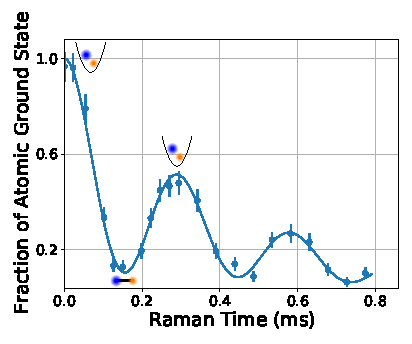
\includegraphics[width=5.5cm]{
              figures/raman_transfer_rabi_annotate.pdf}};
        }
        \visible<6-> {
          \node[below, text width=5.9cm, align=center] at (-3.5, 3.4)
          {
            \begin{itemize}
            \item Transferred $63\%$ of ground state atom to molecule.
            \item<7-> Single molecule spin state
            \item<7-> $>\!50\%$ of molecule\\
              in motional ground state.
            \item<8-> Limited by molecule lifetime
            \end{itemize}
          };
        }
        \visible<6-7> {
          \node[below] at (-3.2, -0.3) {\includegraphics[width=5.3cm]{
              figures/raman_transfer_2d_mol.pdf}};
        }
        \visible<8-> {
          \node[below] at (-3.5, -0.5) {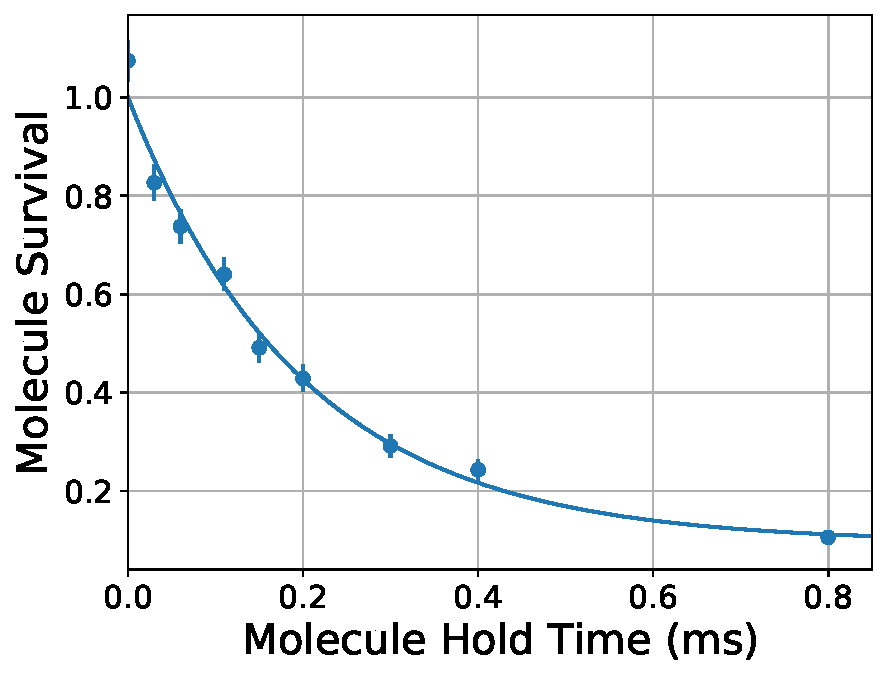
\includegraphics[width=5cm]{
              figures/raman_transfer_fit_two_ase_mol_time.pdf}};
        }
      \end{tikzpicture}
    \end{center}
  \end{adjustwidth}
\end{frame}
\fi

%% ASE
% The first one is from the laser, which is, in fact, already mostly taken care of
% in the some of the data above as I'll explain shortly. __(>>20>>)__
% So it turns out that in additional to the desired frequency,
% the diode laser we use to generate the tweezer and Raman beams
% also has a very broad band spectrum due to amplified spontaneous emission or ASE.
% This is something that we knew before and everyone else we asked also know about it
% but it was surprisingly hard for us to find quantitative information about it.
% __(65/)__

% Furtunately, we found a very sensitive optical spectrum analyser,
% thanks to the Doyle group and, as legend has it,
% Yicheng who basically rescued it from a trash dump.
% This allows us to actually see the ASE in action.
% So here you see what we got from the laser directly,
% the band here is the desired frequency,
% but in additional to that we also saw this broad spectral feature
% that spans tens of nanometers and can couple resonantly to many excited states
% and cause significant scattering.
% __(66/)__

% Furtunately though, since this is a well known problem,
% it was actually easer to find a solution than to measure it. __(>>)__
% It turns out that people makes these 3D Bragg grating with GHz's bandwidth
% and it's a perfect solution to clean up the ASE.
% We got one from Ondax/Coherent with a line width of about 30 GHz
% and __(>>)__ as you can see in this spectrum after the filter,
% the ASE is basically completely gone.
% We move on to test it with our molecule __(>>)__ and the result is shown on this plot.
% __(67/)__

% On the x axis here I'm plotting the Raman Rabi frequency
% and the y axis the scattering rate we measured.
% The bottom right corner corresponds to higher Rabi frequency
% and low scattering which is good
% and the top left corner corresponds to bad transfer efficiency.
% A few points for different tweezer power and filter contiditions are shown,
% and we can clearly see that with a filter added to clean up the laser,
% the points are closer to the bottom right and the transition efficiency is improved.
% __(68/)__

% But this is actually not the end of it. __(>>)__
% We added this filter basically right after our laser
% as shown in this very simplified schematic
% but we were told by the Lukin group that the fiber can cause a very similar effect as well.
% So we added a second filter after the fiber roughly like this __(>>)__
% and we can see the new result here.
% __(69/)__

% For various reasons we were only able to take one point in this configuration
% and it's not completely tuned up either.
% Still you can clearly see that the new point is better
% than any of the previously measured ones.
% This green point is actually the condition where we took the Rabi oscillation
% that I showed you earlier so most of the noise should be removed already.
% However, there are still a few related improvements we can do on that setup
% to ensure that we have eliminated the technical noises as much as possible.
% __(70/49:40)__
\ifSlide{raman_transfer_ase}
\begin{frame}[t]{Amplified Spontaneous Emission (ASE)}
  \vspace{-0.5cm}
  \begin{center}
    \begin{tikzpicture}
      \node at (-3, 2) {
        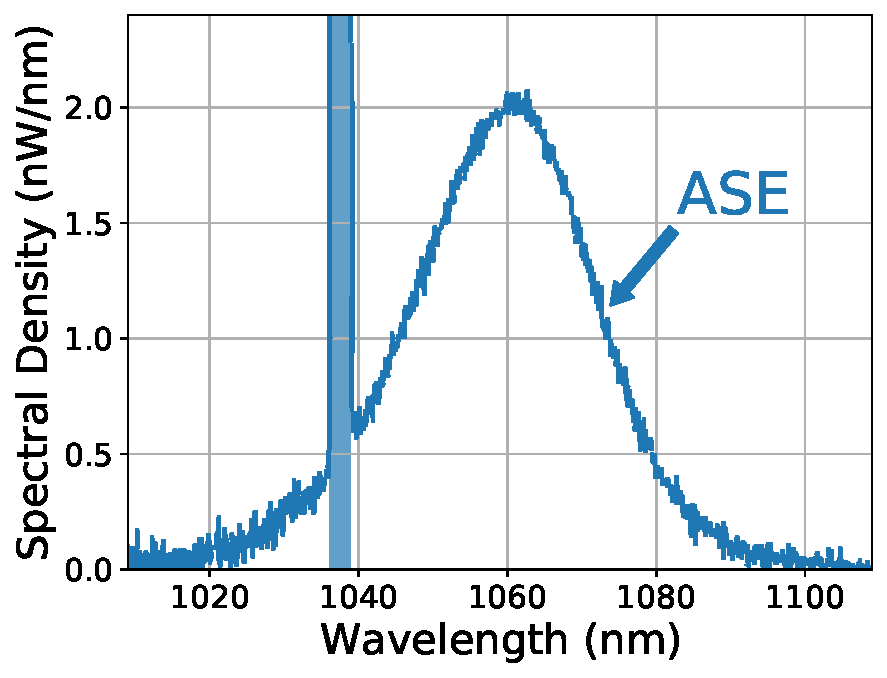
\includegraphics[width=5cm]{figures/raman_transfer_spectrum_prefilter.pdf}};
      \visible<2-4>{
        \begin{scope}[shift={(2, 2)}]
          \draw[red,line width=1.6,mid arrow]
          ({1.7 * cos(40)}, {1.7 * sin(40)}) node[right] {Input} -- (0, 0);
          \draw[red,line width=0.7,mid arrow]
          (0, 0) -- ({-1.2 * cos(40)}, {-1.2 * sin(40)}) node[below] {\small ASE};
          \draw[red,line width=1.6,mid arrow]
          (0, 0) -- node[below,pos=0.6] {Clean Light} (3, 0);
          \drawmirror[line width=8,gray!60!white]{(0, 0)}{0.5}{110};
          \node[rotate=20] at (-0.2, 0.7) {Filter};
        \end{scope}
      }
      \visible<3->{
        \node at (-3, -2) {
          \includegraphics[width=5cm]{figures/raman_transfer_spectrum_postfilter.pdf}};
      }
      \visible<4-5>{
        \node at (3, -2) {
          \includegraphics[width=5cm]{figures/raman_transfer_gamma_vs_omega_0-1.pdf}};
      }
      \visible<5->{
        \begin{scope}[shift={(3, 2)}]
          \draw[red,line width=1.6,mid arrow]
          ({-2.5 + 1.7 * cos(40)}, {-0.5 + 1.7 * sin(40)}) node[above] {Laser}
          -- (-2.5, -0.5);
          \draw[red,line width=1.6,mid arrow] (-2.5, -0.5) -- (-0.65, -0.5);

          \drawmirror[line width=8,gray!60!white]{(-2.5, -0.5)}{0.5}{110};
          \node[rotate=20] at (-2.7, 0.2) {Filter 1};

          \draw[line width=1.2]
          (-0.65, -0.5) --
          plot[domain={(-180 - 360 + 90):(180 + 360 + 90)},smooth,variable=\x,samples=2000]
          ({0.5 * cos(\x) + 0.0003 * \x}, {0.5 * sin(\x)}) -- (0.65, -0.5);

          \node[above] at (0, 0.5) {Fiber};

          \draw[red,line width=1.6,mid arrow] (0.65, -0.5) -- (2.0, -0.5);

          \visible<6->{
            \draw[red,line width=1.6,mid arrow]
            (2.0, -0.5) -- ({2.0 - 1.7 * cos(40)}, {-0.5 - 1.7 * sin(40)});

            \drawmirror[line width=8,gray!60!white]{(2.0, -0.5)}{0.5}{110};
            \node[rotate=20] at (2.2, -1.2) {Filter 2};
          }
        \end{scope}
        \visible<6->{
          \node at (3, -2) {
            \includegraphics[width=5cm]{figures/raman_transfer_gamma_vs_omega_0-2.pdf}};
        }
      }
      \visible<4->{
        \node[pyplotc3] at (1.7, -0.4) {\Large \bf Bad};
        \node[pyplotc2] at (4.8, -3.05) {\Large \bf Good};
      }
    \end{tikzpicture}
  \end{center}
\end{frame}
\fi

%% Two-Photon
% The second potential loss mechanism is a two-photon scattering process. __(>>21>>)__
% So the source I just talked about is mostly what we called background scattering
% and is not very sensitive to the tweezer frequency.
% On the other hand, we can also plot the tweezer frequency **dependent** part
% of the scattering after measuring it at a few different frequencies as shown here.
% We can see that this scattering fits slightly better to the tweezer power squared
% which suggests that this could be a two photon scattering process
% and in that case it could account for almost all the scattering
% with the two filters setup. __(>>)__
% One likely source of this scattering is a Raman process
% that couples the molecular state to the motionally excited state of atoms
% in a different spin state, shown in green.
% Currently we can only do a rough esitmate for this process
% and the result confirms that this is indeed a fine candidate
% depending on the value of a few parameters that we can't exactly determine yet.
% __(71/50:55)__

% Combining these two sources, we believe we have accounted for
% the majority of the scattering that we saw
% and both of these can be reduced either via technical improvements
% or by changing the state selections
% so we should be able to increate the transfer efficiency significantly in the future.
% __(72/51:15)__
\ifSlide{raman_transfer_two_photon}
\begin{frame}{Two-Photon Scattering}
  \begin{center}
    \begin{tikzpicture}
      \node[align=center] at (-3, 0.5) {
        \small Detuning Dependent Scattering\\
        \includegraphics[width=5cm]{figures/raman_transfer_scatter_scaling_mol_diff.pdf}};
      \visible<2->{
        \begin{scope}[shift={(0, -0.5)}, scale=0.8]
          \draw[->,>=stealth,line width=1.2] (0.5, -2.5) --
          node[above,rotate=90] {Energy} (0.5, 5.5);
          \draw[->,>=stealth,line width=1.2] (0.5, -2.5) --
          node[below] {Internuclear Distance} (8, -2.5);

          \draw[line width=1.1,cyan!85!blue]
          plot[samples=200,domain=0.96:7,variable=\x]
          ({(\x + 0.25) * 0.7}, {(6.8*\x^(-3.4)-6.5*\x^(-1.7)) * 1.3 + 2.5});
          \node[cyan!85!blue] at (4, 1.5) {\scriptsize Spin State 1};

          \draw[line width=1.1,green!80!black]
          plot[samples=200,domain=0.96:11,variable=\x]
          ({(\x + 0.25) * 0.7}, {(6.8*\x^(-3.4)-6.5*\x^(-1.7)) * 1.3 + 0.5});
          \node[green!80!black] at (6.5, 0) {\scriptsize Spin State 2};

          \draw[black!40,dashed,line width=1] ({5 * 0.7}, -1 * 1.3 + 7.5) --
          ({8 * 0.7}, -1 * 1.3 + 7.5);

          \draw[cyan!85!blue] ({(1.0793 + 0.25) * 0.7}, -0.28 * 1.3 + 2.5) -- ({(6 + 0.25) * 0.7}, -0.28 * 1.3 + 2.5);
          \mytweezer.drawNaAtom(4.08 * 0.7, -0.19  * 1.3 + 2.5, 0.12)
          \mytweezer.drawCsAtom(4.25 * 0.7, -0.19  * 1.3 + 2.5, 0.10)

          \fill[green!80!black,opacity=0.2] (7.5 * 0.7, 0.5) rectangle (10.5 * 0.7, 3.5);
          \draw[green!80!black,dashed] (7.5 * 0.7, 0.5) -- (11 * 0.7, 0.5);
          \draw[->,green!80!black,line width=0.8] (10.7 * 0.7, 0.5) --
          node[below,rotate=90] {\scriptsize Motional Continuum} (10.7 * 0.7, 4.5);

          \draw[fullsnakearrow,red,line width=0.8]
          (8.7 * 0.7, -0.19  * 1.3 + 2.5) -- (7.7 * 0.7, -0.19  * 1.3 + 2.5);
          \draw[fullsnakearrow,red,line width=0.8]
          (9.3 * 0.7, -0.19  * 1.3 + 2.5) -- (10.3 * 0.7, -0.19  * 1.3 + 2.5);

          \mytweezer.drawNaAtom(8.7 * 0.7, -0.19  * 1.3 + 2.5, 0.12)
          \mytweezer.drawCsAtom(9.3 * 0.7, -0.19  * 1.3 + 2.5, 0.10)

          \draw[->,>=stealth,blue!50!orange,line width=0.8] (4.165 * 0.7, -0.12 * 1.3 + 2.5)
          -- ({6.5 * 0.7}, -1 * 1.3 + 7.5);

          \draw[->,>=stealth,blue!50!orange,line width=0.8] ({6.55 * 0.7}, -1 * 1.3 + 7.5)
          -- (9 * 0.7, -0.12 * 1.3 + 2.5);
        \end{scope}
      }
    \end{tikzpicture}
  \end{center}
\end{frame}
\fi

\section{Conclusion}
%% Conclusion
% So as conclusion, __(>>22>>)__ we designed and built an experiment for a new quantum platform
% based on trapping ultracold molecules in optical tweezers. __(>>)__
% We demonstrated the quantum control on atoms
% by preparing them into a single quantum state __(>>)__
% and use it to measure the interaction between atoms. __(>>)__
% After that, we coherently created a single molecule in the tweezer
% using only optical transitions while maintaining the control we had.
% We believe the efficiency can be further improved. __(>>)__
% Looking ahead, the molecules needs to be transfered to the rovibronic ground state
% to turn on the strong interaction
% and we have actually just demostrated it starting from FB molecule in a separate setup.
% __(73/52:10)__
\ifSlide{conclusion}
\begin{frame}[t]{Conclusion and outlook}
  \vspace{-0.5cm}
  \begin{columns}
    \column{6.25cm}
    \begin{itemize}
    \item New quantum platform based on ultracold molecules in tweezers
    \item<2-> Full quantum control of atoms in optical tweezers
    \item<3-> Measured interaction between single atoms
    \item<4-> Coherent all-optical creation of single molecucle
    \item<5-> Rovibronic ground state
    \end{itemize}
    \column{5.7cm}
    \visible<5->{
      \vspace{1cm}\\
      \includegraphics[width=5.7cm]{figures/conclusion_ground_raman_annotate.pdf}
    }
  \end{columns}
\end{frame}
\fi

%% Acknowledgement
% __(>>23>>)__ Of course none of the results I just presented would have be possible
% without the contribution and support from many others.
% First, I would like to thank my committee and especially my advisor Kang-Kuen Ni,
% for designing and stearing the experiment
% and for teaching me the way to manage a lab and to do research in general.
% I also want to thank the contribution from other people in our group
% from both the NaCs and KRb teams,
% especially our former members Lee, Nick and Jon who built the experiment from scratch
% and from whom I learnt a lot,
% and the current members Kenneth, Wang Yu and Fang,
% who are now leading the experiment to the next level. __(>>)__
% Being in Harvard and part of CUA is really a blessing to our experiment
% and we have got a lot of help from other groups here
% from inspirations to equipments
% and I have already mentioned a few of these in my presentation.
% __(74/53:15)__
\ifSlide{acknowledgement_lab}
\begin{frame}
  \begin{center}
    \begin{tikzpicture}
      %% PI
      \node[align=center] at (-2.5, -0.9) {PI};
      \node[below,align=center, execute at begin node=\setlength{\baselineskip}{7.5pt}]
      at (-1, -0.1) {\includegraphics[height=1.5cm]{figures/acknowledgement_kangkuen.jpg}\\
        \scriptsize Kang-Kuen Ni};

      %% NaCs
      \node[align=center] at (-3, -3.1) {NaCs\\Team};
      \node[below,align=center, execute at begin node=\setlength{\baselineskip}{7.5pt}]
      at (-1.5, -2.2){\includegraphics[height=1.5cm]{figures/acknowledgement_kenneth.jpg}\\
        \scriptsize Kenneth\\\scriptsize Wang};
      \node[below,align=center, execute at begin node=\setlength{\baselineskip}{7.5pt}]
      at (0.0, -2.2) {\includegraphics[height=1.5cm]{figures/acknowledgement_wangyu.jpg}\\
        \scriptsize Yu\\\scriptsize Wang};
      \node[below,align=center, execute at begin node=\setlength{\baselineskip}{7.5pt}]
      at (1.5, -2.2) {\includegraphics[height=1.5cm]{figures/acknowledgement_fang.jpg}\\
        \scriptsize Fang\\\scriptsize Fang};
      \node[below,align=center, execute at begin node=\setlength{\baselineskip}{7.5pt}]
      at (3.0, -2.2) {\includegraphics[height=1.5cm]{figures/acknowledgement_jessie.jpg}\\
        \scriptsize Jessie\\\scriptsize Zhang};
      \node[below,align=center, execute at begin node=\setlength{\baselineskip}{7.5pt}]
      at (4.5, -2.2) {\includegraphics[height=1.5cm]{figures/acknowledgement_lewis.jpg}\\
        \scriptsize Lewis\\\scriptsize Picard};
      \node[below,align=center, execute at begin node=\setlength{\baselineskip}{7.5pt}]
      at (6.0, -2.2) {\includegraphics[height=1.5cm]{figures/acknowledgement_will.jpg}\\
        \scriptsize William\\\scriptsize Cairncross};

      % KRb
      \node[align=center] at (-2, -5.3) {KRb\\Team};
      \node[below,align=center, execute at begin node=\setlength{\baselineskip}{7.5pt}]
      at (-0.5, -4.4) {\includegraphics[height=1.5cm]{figures/acknowledgement_lingbang.jpg}\\
        \scriptsize Lingbang\\\scriptsize Zhu};
      \node[below,align=center, execute at begin node=\setlength{\baselineskip}{7.5pt}]
      at (1.75, -4.4) {\includegraphics[height=1.5cm]{figures/acknowledgement_mingguang.jpg}\\
        \scriptsize Mingguang\\\scriptsize Hu};
      \node[below,align=center, execute at begin node=\setlength{\baselineskip}{7.5pt}]
      at (4.0, -4.4) {\includegraphics[height=1.5cm]{figures/acknowledgement_matt.jpg}\\
        \scriptsize Matthew\\\scriptsize Nichols};

      %% Former member
      \node[below,align=center, execute at begin node=\setlength{\baselineskip}{7.5pt}]
      at (-3.5, -6.6) {\includegraphics[height=1.5cm]{figures/acknowledgement_lee.jpg}\\
        \scriptsize Lee Liu\\\tiny Postdoc @JILA};
      \node[below,align=center, execute at begin node=\setlength{\baselineskip}{7.5pt}]
      at (-2.05, -6.6) {\includegraphics[height=1.5cm]{figures/acknowledgement_nick.jpg}\\
        \scriptsize Nick Hutzler\\\tiny AP @Caltech};
      \node[below,align=center, execute at begin node=\setlength{\baselineskip}{7.5pt}]
      at (-0.4, -6.6) {\includegraphics[height=1.5cm]{figures/acknowledgement_jon.jpg}\\
        \scriptsize Jonathan Hood\\\tiny AP @Purdue};
      \node[below,align=center, execute at begin node=\setlength{\baselineskip}{7.5pt}]
      at (1.0, -6.6) {\includegraphics[height=1.5cm]{figures/acknowledgement_eliot.jpg}\\
        \scriptsize Eliot\\\scriptsize Fenton};
      \node[below,align=center, execute at begin node=\setlength{\baselineskip}{7.5pt}]
      at (2.5, -6.6) {\includegraphics[height=1.5cm]{figures/acknowledgement_yenwei.jpg}\\
        \scriptsize Yen-Wei Lin\\\tiny Intelon Optics};
      \node[below,align=center, execute at begin node=\setlength{\baselineskip}{7.5pt}]
      at (4.0, -6.6) {\includegraphics[height=1.5cm]{figures/acknowledgement_yu.jpg}\\
        \scriptsize Yu Liu\\\tiny Postdoc @NIST};
      \node[below,align=center, execute at begin node=\setlength{\baselineskip}{7.5pt}]
      at (5.5, -6.6) {\includegraphics[height=1.5cm]{figures/acknowledgement_andrei.png}\\
        \scriptsize Andrei\\\scriptsize  Gheorghe};
      \node[below,align=center, execute at begin node=\setlength{\baselineskip}{7.5pt}]
      at (6.9, -6.6) {\includegraphics[height=1.5cm]{figures/acknowledgement_david.jpg}\\
        \scriptsize David Grimes\\\tiny Instructor @MIT};

      \visible<2->{
        \node[below] at (2, -0.1) {
          \includegraphics[height=1.5cm]{figures/acknowledgement_harvard.png}};
        \node[below] at (5, -0.1) {
          \includegraphics[height=1.5cm]{figures/acknowledgement_cua.png}};
      }
    \end{tikzpicture}
  \end{center}
\end{frame}
\fi

% __(>>24>>)__ I've also got a lot of support from outside the lab.
% Of course I have to thank my parents for being my first teachers,
% got me interested in science
% and supports me through all the difficulties during my PhD. __(>>)__
% I also want to thank my cousin and her family in New Your City
% who helped me in a number of times when my parents are too far away to reach me.
% I'd like to thank everyone to be here
% and especially all the friends that I've invited to come today
% and this is actually one of the few reasons I'm really glad this is held online.
% There are of course too many to mention them all,
% but I'd like to mention two groups in particular. __(>>)__
% Thanks to Horizon Aviation and the Julia project
% which I spent a lot of my spare time with.
% It really made my PhD time much more fun and fruitful than it would have been otherwise.
% __(75/54:10)__

% __(>>)__ With that, this is the end of my talk,
% thank you for your attention,
% and I'll leave it on these beautiful Rabi floppings for our molecule formation.
% __(76/54:20)__
\ifSlide{acknowledgement_other}
\begin{frame}
  \begin{center}
    \begin{tikzpicture}
      \node at (-3, 2.2) {
        \includegraphics[width=5.3cm]{figures/acknowledgement_family.jpg}};
      \visible<2->{
        \node at (-3, -2.2) {
          \includegraphics[width=5.3cm]{figures/acknowledgement_cousin.jpg}};
      }
      \visible<3->{
        \node at (3, 2.2) {
          \includegraphics[width=5cm]{figures/acknowledgement_nha.jpg}};
        \node at (4.4826, 3.5) {
          \includegraphics[width=2cm]{figures/acknowledgement_nha_logo.png}};
        \node at (3, -2.2) {
          \includegraphics[width=4cm]{figures/acknowledgement_julia.pdf}};
      }
      \visible<4->{
        \fill[white,opacity=0.94] (-5.7, -4.5) rectangle (5.55, 4.3);
        \node at (0, 3.0) {\LARGE \bf \usebeamercolor[fg]{frametitle}{Thanks for your attention}};
        \node at (-2.8, -0.5) {\includegraphics[width=5.8cm]{
            figures/raman_transfer_rabi_annotate.pdf}};
        \node at (3.1, -0.7) {\includegraphics[width=5.8cm]{
            figures/conclusion_ground_raman_annotate.pdf}};
      }
    \end{tikzpicture}
  \end{center}
\end{frame}
\fi

\begin{frame}{}
\end{frame}

\begin{frame}{}
\end{frame}

%% Backup slides

% Our experiment starts with trapped atoms in tweezers.
% People have demonstrated before us.
% It sounds simple but turns out to be anything but.

% Well, Cs is fine.
% Got without too much effort.
% But Na is not.
% A few properties.
% * Low vapor pressure (fewer atoms to load from)
% * Broad linewidth (higher Doppler temperature)
% * Low mass (move faster and higher recoil velocity/energy)
% * Small HF structure (6 line width, worse PG cooling)

% Fine just need deeper trap but run into the real issue
% * Light shift
% In order to load, need cooling in the tweezer
% However, since we need such a deep trap, light shift turns off the cooling
% Got stuck in an awkward situation where a shallow trap can keep the cooling work but
% can't hold the atom while a deeper trap can hold the atom but the atom doesn't want to come in.

% Tried a bunch of ways (turn trap around atom, two wavelengths to cancel the trap)
% before Nick came up with a genius/crazy idea that people have used on large ODT.

% See laser cooling relies on scattering that happens at a rate of tens of MHz
% OTOH, the tweezer is only needed for trap motion that happens ~ few hundred kHz.
% Means that if we switch the tweezer on and off. .....

% Tried on Cs
% Essentially made a magic trap.

% Then tried on Na, it worked.
% Na live atom.
\ifSlide{loading_intro}
\begin{frame}{Single Atom in Tweezer}
  \begin{columns}[t]
    \column{5cm}
    \begin{block}{}
      \begin{itemize}
      \item Previously done with Rb
      \item<2-> Works for Cs
      \item<3-> Doesn't work for Na
      \end{itemize}
    \end{block}
    \column{6cm}
    \begin{center}
      \begin{tikzpicture}
        \visible<2> {
          \node at (0, 0)
          {\includegraphics[width=6cm]{figures/loading_cs_histogram.png}};
        }
        \visible<3> {
          \node at (0, 0)
          {\includegraphics[width=5cm]{figures/loading_na_noatom.png}};
        }
        \visible<4> {
          \node[text width=6cm] at (0, 0) {
            \begin{block}{Issues with Na}
              \begin{itemize}
              \item Low vapor pressure
              \item Broad linewidth
              \item Low mass
              \item Small hyperfine structure
              \end{itemize}
            \end{block}
          };
        }
      \end{tikzpicture}
    \end{center}
  \end{columns}
\end{frame}
\fi

\ifSlide{loading_lightshift}
\begin{frame}{Real Issue with Na: Light Shift}
  \vspace{-1cm}
  \begin{columns}
    \column{5.7cm}
    \begin{center}
      \only<-3>{\includegraphics[width=5.5cm]{figures/loading_light_shift.png}}
      \only<4->{
        \begin{block}{Trap modulation}
          Alternate between trap and resonant {\small (cooling and imaging)} light
          at $2.5$\ MHz\\
          {\small $f_{trap}=100\sim500$\ kHz}\\
          {\small $\Gamma=2\pi\times 10$\ MHz}
        \end{block}
        \includegraphics[width=5cm]{figures/loading_switching.png}
      }
    \end{center}
    \column{5.8cm}
    \begin{center}
      \begin{tikzpicture}
        \visible<2-4>{
          \node[align=center] at (0, 0) {Cs single atom imaging\\
            \includegraphics[width=5.5cm]{figures/loading_det_vs_photon_dc.png}};
        }
        \visible<3-5>{
          \node[align=center, text width=5cm] at (0, -4.5) {
            \begin{block}{}
              \begin{itemize}
              \item Low imaging signal
              \item No cooling in tweezer
              \end{itemize}
            \end{block}
          };
        }
        \visible<5->{
          \node[align=center] at (0, 0) {Cs single atom imaging\\
            \includegraphics[width=5.5cm]{figures/loading_det_vs_photon_ac.png}};
        }
        \visible<6->{
          \node at (0, -4.5)
          {\includegraphics[width=4cm]{figures/overview_single_atom.png}};
        }
      \end{tikzpicture}
    \end{center}
  \end{columns}
\end{frame}
\fi

%% Another thing we can measure is the FB resonance
% Better prediction than before.
\ifSlide{fb}
\begin{frame}[t]{Na (1, -1) Cs (3, -3) Feshbach resonance}
  \only<1>{
    \begin{center}
      \includegraphics[height=7cm]{figures/fb_chamber1_5.jpg}
    \end{center}
  }
  \only<2->{
    \begin{center}
      \includegraphics[width=10cm]{figures/fb_resonance.pdf}\\
      \vspace{0.5cm}
    \end{center}
  }
  \only<3->{
    \begin{center}
      \begin{tabular}{|c|p{1.9cm}|p{1.9cm}|}
        \hline
        &$s$-wave&$p$-wave\\\hline
        Predicted {\tiny (based on interaction shift)\footnote{In collaboration with Bo Gao}}&$663$ G&$799$ G\\\hline
        Measured&$652(3)$ G&$791.2(2)$ G\\\hline
      \end{tabular}
    \end{center}
  }
\end{frame}
\fi

% Raman transfer obviously need some information about the excited state
% So that's what we set out to measure first. (i.e. PA spectroscopy)

% We really have the most textbook system to do this measurement.
% We only have two atoms
% We know the initial state
% We shine some light on it, which might create some excited state molecule that
% falls down to some states that we can't see.
% We know the final state

% Full state info, improve signal-to-noise

% We start with near threshold since the lines are denser/easier to see.
% Single body - flat
% Two body - peaks
% Agreement with the theory/see new lines

% Also found deeper lines afterwards with very similar signal so I'm not showing it here.

% Now we know the excited states.
% After measuring this line, we can use add another beam in order to find
% the ground molecular state.
% With one laser parked on the PA resonance, we can scan the frequency of the other.
% When the difference between the two lasers match ... we can create a EIT and stops the
% PA process ...

% We scanned around the theoritical prediction between 200-300 MHz and indeed found the resonance.
\ifSlide{pa_eit}
\begin{frame}[t]{\alt<-4>{Photoassociation (PA) Spectroscopy}{Electromagnetically Induced Transparency (EIT) Spectroscopy}}
  \vspace{-0.4cm}
  \begin{center}
    \begin{tikzpicture}
      \begin{scope}[shift={(-4.3, -3.3)}, scale=0.7]
        \draw[->,>=stealth,line width=1.2] (0, 0) -- (0, 8);
        \node[above,rotate=90] at (0, 4) {Energy};
        \draw[->,>=stealth,line width=1.2] (0, 0) -- (8, 0);
        \node[below] at (4, -0.1) {Internuclear Distance};

        \draw[cyan!85!blue] (1.0269 + 0.25, 2.5) -- (7.25, 2.5);

        \draw[line width=1.1,cyan!85!blue]
        plot[samples=200,domain=1:7,variable=\x]
        ({\x + 0.25}, {6.8*\x^(-3.4)-6.5*\x^(-1.7) + 2.5});
        \node[cyan!85!blue] at (3.75, 1.0) {${\rm a}^3\Sigma^+$};

        \draw[line width=1.1,red]
        plot[samples=200,domain=1:7.5,variable=\x]
        ({\x - 0.75}, {9.2*\x^(-2.5)-9.0*\x^(-1.3) + 7.5});
        \node[above right,red] at (0.55, 7.2) {${\rm c}^3\Sigma^+$};

        \draw[red] (1.1102 - 0.75, -0.7720 + 7.5) -- (6 - 0.75, -0.7720 + 7.5);
        \draw[red] (1.1576 - 0.75, -1.0595 + 7.5) -- (4.5 - 0.75, -1.0595 + 7.5);

        \mytweezer.drawNaAtom(6.55, 2.6, 0.12)
        \mytweezer.drawCsAtom(7.05, 2.6, 0.10)

        \draw[->,>=stealth,blue!50!orange,line width=0.8] (6.8, 2.7) -- (4.5 - 0.75, -0.85 + 7.5);

        \only<5->{
          \draw[cyan!85!blue] (1.0793 + 0.25, -0.4631 + 2.5) -- (4.5 + 0.25, -0.4631 + 2.5);
          \draw[cyan!85!blue,<->,>=stealth] (3.5, 2.5) -- ++(0, -0.4631) node[midway, left]
          {\tiny $\delta$};
          \mytweezer.drawNaAtom(4.08, 2.15, 0.12)
          \mytweezer.drawCsAtom(4.25, 2.15, 0.10)
          \draw[->,>=stealth,green!80!black,line width=0.8] (4.165, 2.25) -- (4.45 - 0.75, -0.85 + 7.5);
        }
      \end{scope}
      \visible<2-4>{
        \node[text width=5cm] at (4.2, -1) {
          \begin{block}{Single Atom PA}
            \begin{itemize}
            \item Clean initial state
            \item Narrow excitation laser
            \item Final state detection
            \end{itemize}
          \end{block}
        };
      }
      \visible<3>{
        \node at (3, 3) {\includegraphics[width=8cm]{figures/pa_shallow_1b.pdf}};
      }
      \visible<4>{
        \node at (3, 3) {\includegraphics[width=8cm]{figures/pa_shallow.pdf}};
      }
      \visible<6>{
        \node at (4, 2.5) {\includegraphics[width=5cm]{figures/pa_eit.png}};
      }
    \end{tikzpicture}
  \end{center}
\end{frame}
\fi

\end{document}
